\chapter{Ein Anhangskapitel}

Hier könnte ein Anhang stehen, falls Sie z.\,B.\ Code, Konstruktionszeichnungen oder Ähnliches mit in die Arbeit bringen wollen.
Im Normalfall stehen jedoch alle Ihre Resultate im Hauptteil der Bachelorarbeit und ein Anhang ist überflüssig.

\section{Einkristalloberflächen}
        Die geordneten Strukturen eines Einkristalls kommen durch die Wechselwirkung der Elektronen zwischen den einzelnen Atomen.
        So ergibt sich eine periodische Anordnung der Atome im thermischen Gleichgewicht.
        Dabei sind die Atome nicht komplett starr an ihre Plätze gebunden, sondern führen kleine Schwingungen um diesen aus.
        Mit der Temperatur sinkt auch die Auslenkung.
        Dieses Wechselspiel der strukturellen Ordnung findet sich auch in der elektronischen Struktur wieder.
                
        Wird ein Einkristall entlang einer Kristalleben durchschnitten so ergibt sich eine Oberfläche.
        Die Ebene erhält den Namen der Indizes des auf ihr senkrecht stehenden Gittervektors $r_{hkl}$, also $(hkl)$.
        Als Oberfläche werden die oberen Atomlagen definiert, die sich in der geometrischen und/oder chemischen Art von der des Volumens unterscheiden~\cite{Fauster}.
        Aufgrund der nun fehlenden Bindungen nach oben ergeben sich neue elektronische und geometrische Eigenschaften.
        So kann es zu lateralen und transversalen Verschiebungen gegenüber der volumenartigen Struktur, so genannte Rekonstruktionen und Relaxation kommen.
        Dabei ordnen sich die Atome um, um damit einen energetisch günstigeren Zustand zu erhalten.
    
        Wie im Volumenkristall kann die Oberfläche durch eins von fünf Bravais-Gittern beschrieben werden, wobei auf jedem Gitterpunkt eine atomare Basis gesetzt wird.
        Die Punkte dieses zweidimesionalen Gitters lassen sich durch den Gittervektor
        \begin{equation}
            \vec{r}_{nm} = n \vec{a}_1 + m \vec{a}_2
            \label{eqn:Gittervek}
        \end{equation}
        mit $n,m \in \mathbb{Z}$ und den Vektoren der Einheitszelle $\vec{a}_1, \vec{a}_2$ beschreiben.
        Geimeinsam legt das Bravais-Gitter und die atomare Basis die Symmetrien der Oberfläche fest.
    
        Durch die Anlagerung von Adsorbaten können Symmetrien der Oberfläche verloren gehen.
        Die Struktur der Adsorbate relativ zur Oberfläche wird Überstruktur genannt.
        Durch den meist größeren Abstand der Adsorbate untereinander als der Basen des Substrates ergibt sich auch eine größere Einheitszelle.
        Beim Schneiden der Einkristalle um eine Oberfläche zu erhalten können sich unter anderem auch Stufen ausbilden.
        Vermehrt treten diese Stufen bei hochindizierten Oberflächen auf, wobei einzelne Terrassen dann eine niedrigindizierte Oberfläche darstellen~\cite{Fauster}.
        Diese Stufen oder auch Defekte in der Oberfläche bilden Keimzellen für Anlagerung von Adsorbaten.
        Um die Überstruktur des Adsorbate zu beschreiben wird die von ihnen aufgespannte Einheitszelle aus den Gittervektoren des Substrats rekosntruiert.
        Die Gittervektoren des Übergitters $\vec{b}_1, \vec{b}_2$ lassen sich dann als Matrixschreibweise darstellen.
        Damit ergibt sich auch die Überstrukturmatrix $C$ mit 
        \begin{equation}
            \begin{pmatrix}
                \vec{b}_1 \\
                \vec{b}_2 \\
            \end{pmatrix}
            = 
            \begin{pmatrix}
                C_{11} & C_{12} \\
                C_{21} & C_{22} \\
            \end{pmatrix}
            \begin{pmatrix}
                \vec{a}_1 \\
                \vec{a}_2 \\
            \end{pmatrix}.
        \end{equation}
        Relative Verschiebungen zum Substrat bleiben dabei ohne Beachtung, es zeigt nur die Periodizität der Struktur an.
        Ferner kann es zur Aubildung verschiedener Domänen kommen, besonders dann, wenn die Symmetrie des Übergitters kleiner als die des Substrates ist~\cite{Fauster}.
        Einzelne Domänen weisen Symmetrie äquivalente Anordnungen auf, häufug handelt es sich nur umgedrehte Einheitszellen.
        Nicht nur Adsorbatebedeckungen lassen sich durch diese Notation beschreiben, auch die Rekonstruktion der Oberfläche.
        Hierbei sind es keine Adsorbatatome, sondern die Oberflächenatome selbst, die eine neue Struktur ausbilden.
        Die Relaxation, welche die Änderung im Lagenabstand beschreibt kann hingegen nicht durch dies Notation beschrieben werden.
        Sie ist ebenso wie die Rekonstruktion vom Material, der Kristallstruktur und der Oberflächenorientierung abhängig.
        Einige Rekonstruktionen und Relaxation hängen auch vom Präperationsprozess ab, wenn die Oberfläche selbst metastabil ist.
    
        Wie bereits erwähnt hängen geometrische und elektronische Struktur stark zusammen.
        Sodass sich an Oberflächen durch die fehlenden Bindungen die elektronische Struktur verändern kann.
        Die quantenmechanische Beschreibung der Elektronen erlaubt es auch die elektronischen Zustände der Oberfläche durch Quantenzahlen auszudrücken.
        Hier ist $\vec{k}_{||}$ der Wellenzahlvektor der Oberfläche die Ausschlag gebende Größe um die Oberflächenbandstruktur $E(\vec{k}_{||})$ zu beschreiben.
        Ganz besondere Beachtung erhalten die Zustände nahe der Fermikante $E_\text{F}$ die für leitenden Eigenschaften verantwortlich sind.
        Erhaltene Oberflächenbandstruktur kann von der der Volumenbandstruktur abweichen.
        Dies führt zum Teil zu Oberflächenzuständen, die unterscheiden sich energetisch von denen im Volumenkristall und können somit nur in dessen Bandlücke auftreten.
    
        % Ein wichtiger Ansatz für die periodische Struktur der Oberfläche und dessen elektronischen Zustände ist das Bloch Theorem.
        % Die Oberfläche entspricht einer Anordung äquivalenter Punkte welche durch den Gittervektor aus \autoref{eqn:Gittervek} ineinander überführt werden können

        \subsection{Eisen (100) Oberfläche}
            \begin{itemize}
                \item WKF
                \item Symmetrie - p4mm
                \item Gitterkonstante ist $a = \SI{2.862}{\angstrom}$~\cite{springer_database}
                \item bcc Struktur
            \end{itemize}
        
        \subsection{Gold (111) Oberfläche}
            Gold gehört zu den Edelmetallen und kristallisiert in der flächenzentrierten Struktur mit einer Gitterkonstanten von \SI{4.08}{\angstrom}~\cite{Marx}.
            Es ist besonders leitfähig, stabil und wenig reaktiv, dennoch rekosntruiert die Oberfläche in einer Fischgräten-Struktur ($\num{22} \times \sqrt{\num{3}}$)~\cite{5A_3}.
            Die Austrittsarbeit der (111)-Oberfläche wurde dabei auf \SI{5.46}{\electronvolt} bestimmt~\cite{5A_4}.
            Ebenfalls bildet sich auch ein sehr präsenter Oberflächenzustand aus.
            
            Auf Grund der sehr ähnlichen Gitterkonstante zu der des Nickeloxids von nur etwa \SI{2}{\percent} eignet es sich besonders gut als Substrat \cite{NiO_36}.
            \begin{itemize}
                \item Ebenenabstand in Au(111) $d_0 = \SI{2.35}{\angstrom}$.\textbf{\cite{5A_1}}
            \end{itemize}

            Bereits bekannt ist, dass sich auf diesem Substrat das Pentacene anordnet~\cite{5A_1, 5A_3}.
            Die lange Molekülachse liegt dabei parallel zu den Reihen der Goldatome, mit den äußeren Ringen und somit die $\pi$-Orbitale direkt oberhalb eines Goldatoms.
            Diese Positionierung lässt auf eine starke Substrat-Molekül-Interaktion schließen~\cite{5A_3}.
            Bei der Wechselwirkung dieser handelt es sich um Physisorption, was damit auch die Adsorbate-Adsorbat-Wechselwirkung zur Formung der Einheitszelle dominieren lässt~\cite{5A_4}.
            Ferner liegen in einer Monolage flach auf der Oberfläche und einzelne Reihen sind durch eine Reihe Goldatome separiert.
            Allerdings wächst der Pentacenefilm nicht epitaxtisch, sondern in Form von Inseln mit unterschiedlichen Einheitszellen~\cite{5A_3}.

            \begin{figure}
                \centering
                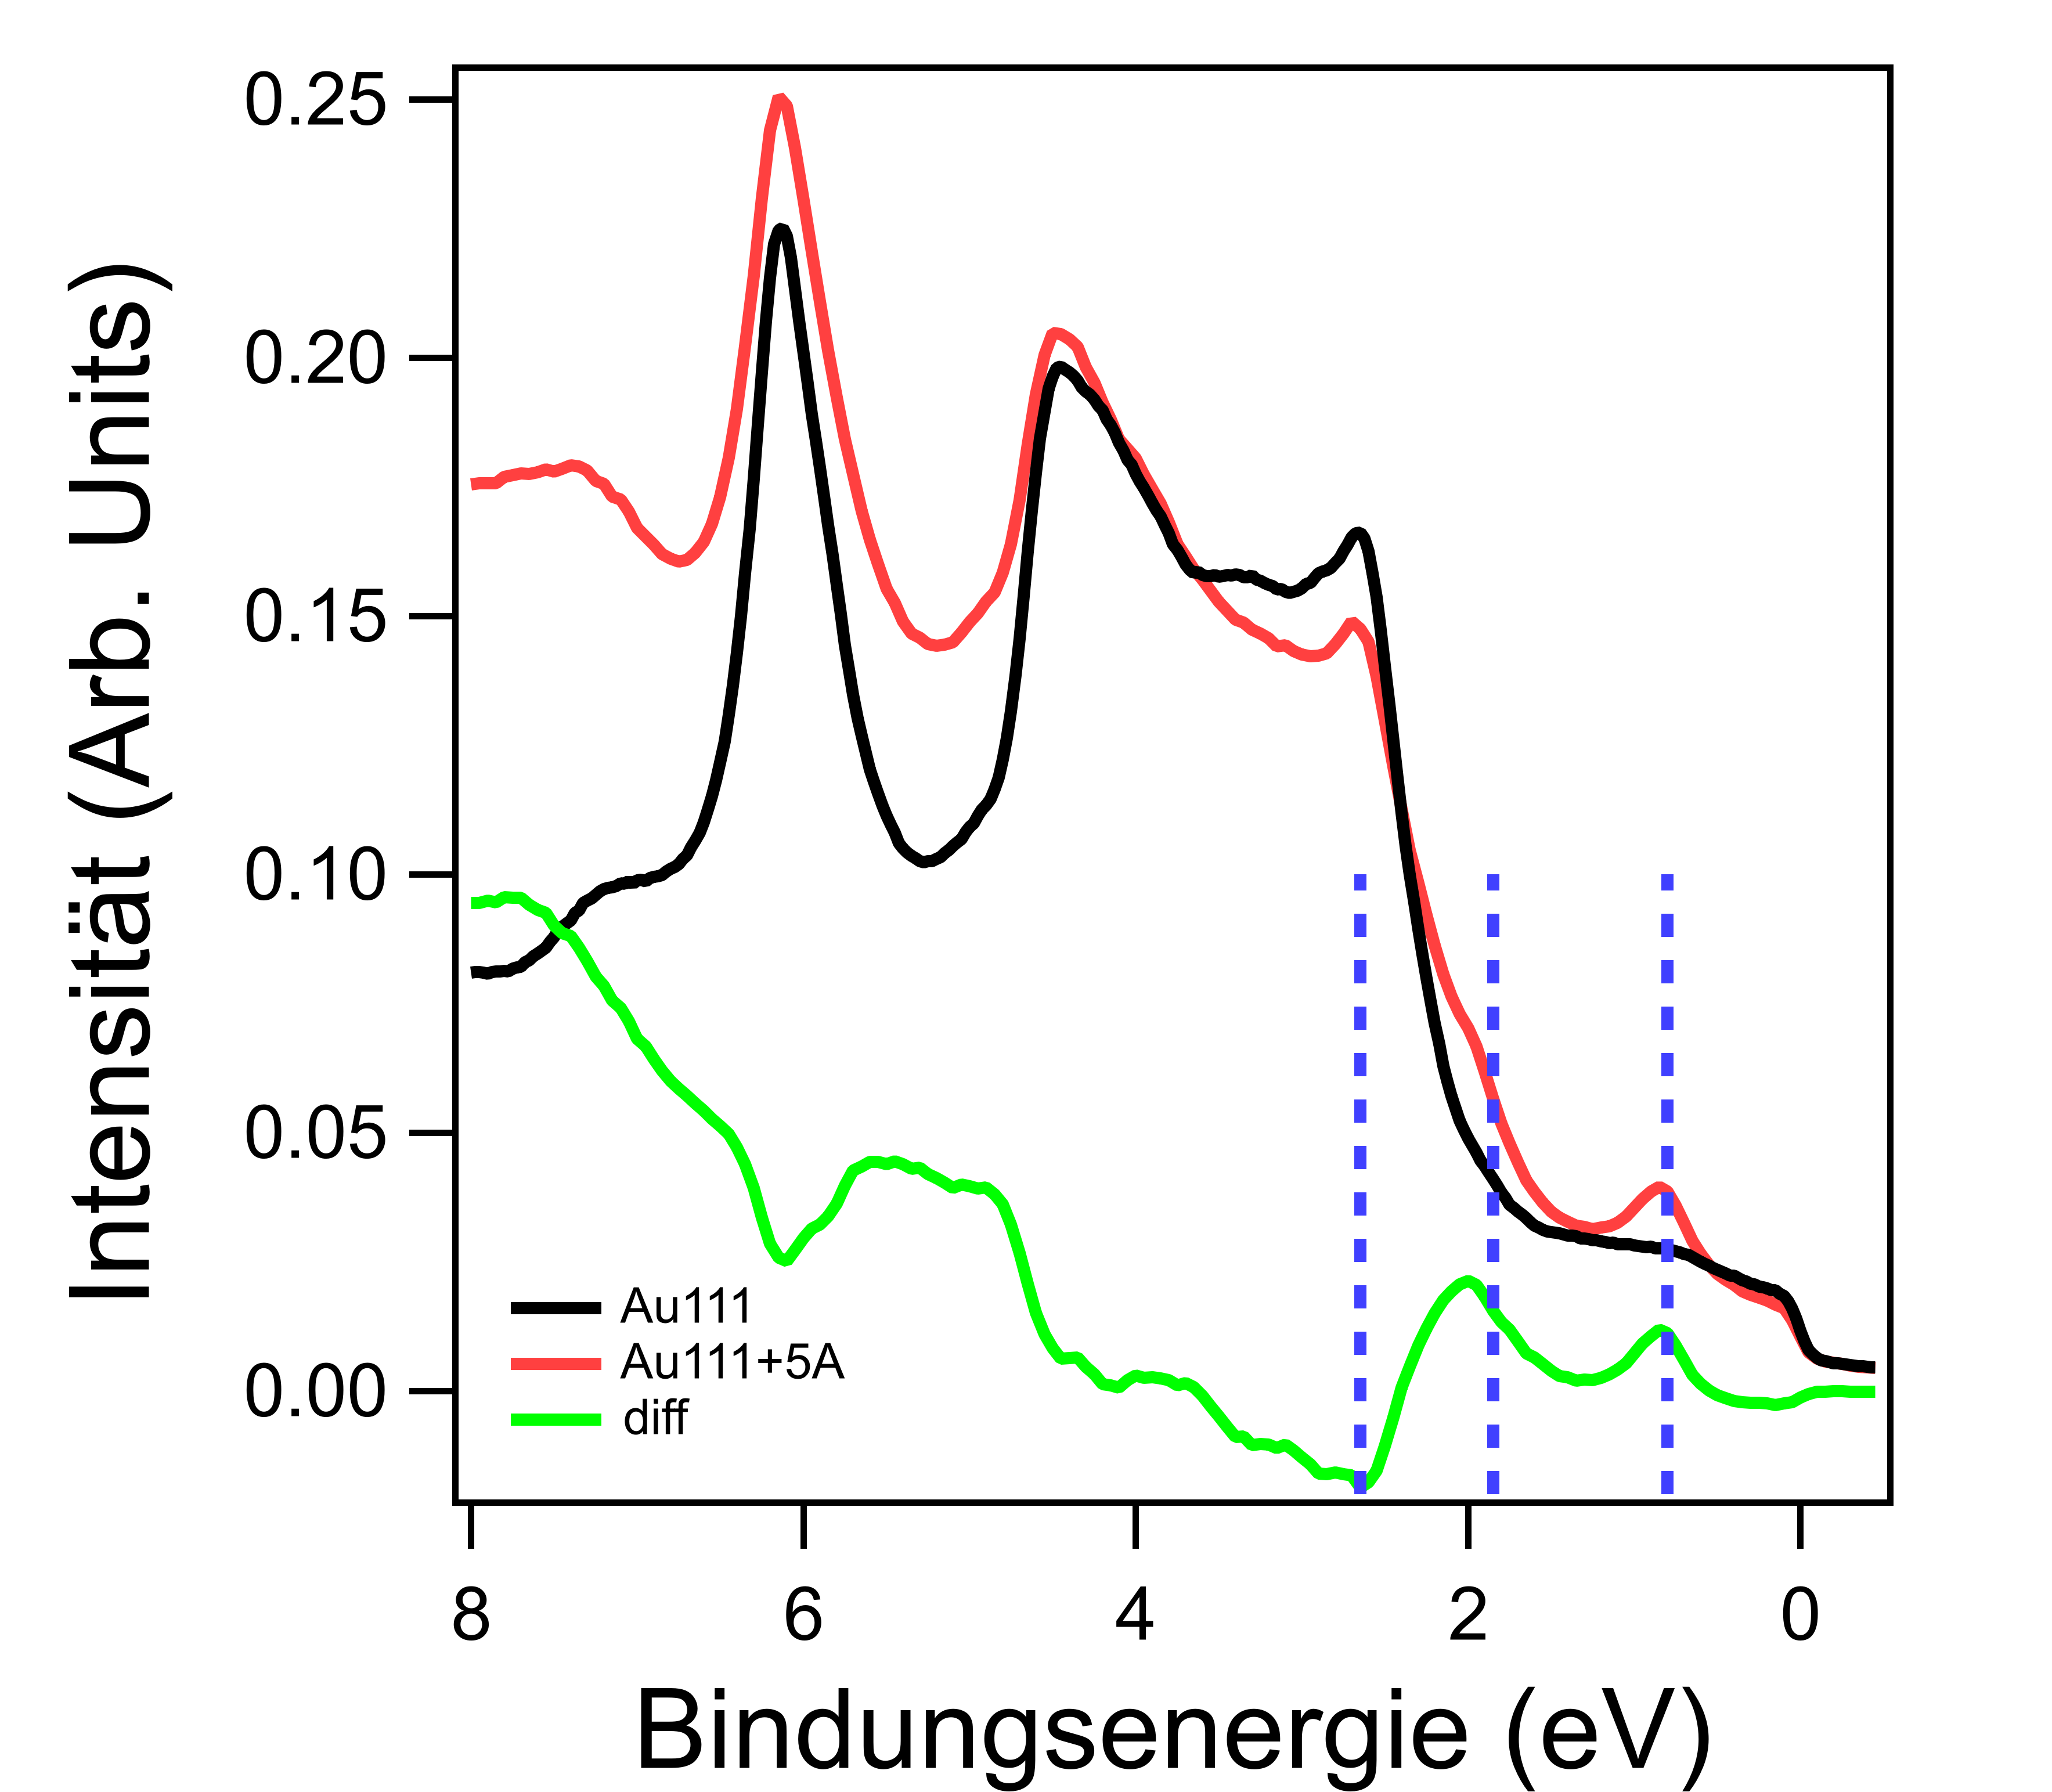
\includegraphics[width=0.5\textwidth]{Au+5A/EDC_Au_5A_mod.png}
                \caption{Die integrierten Spektren für reines Gold, Gold mit einer Monolage Pentacene und deren Differenz.}
                \label{fig:EDC_Au+5A}
            \end{figure}
            Das Goldsubstrat eignet sich ebenfalls zur Kalibrierung der Monolage von Pentacene, da bereits bekannt ist, dass sich diese flach auf der Oberfläche ordnet \cite{5A_1}.
            Bei der Wechselwirkung mit dem Substrat handelt es sich um die Physisorption durch einen Substrat-Molekülabstand von \SI{3.28}{\angstrom} \cite{5A_1}.
            % Es ergibt sich so das LEED-Bild in \autoref{fig:LEED_Au+5A}, was auch die bekannte \textbf{Überstruktur} (5A_1, 5A_5) aufweist.
            Schaut man sich das winkelintegrierte Spektrum im Bereich der Valenzzustände in \autoref{fig:EDC_Au+5A} an, so sind auch deutlich Elemente zu erkennen, die durch die Moleküle hervorgerufen werden.
            Die senkrechten Linien stellen die Punkte da, an denen Bilder mit höherer Statistik aufgenommen wurden und die später zur Molekülorbitalanalyse herangezogen werden.
    
            \begin{figure}
                \centering
                \begin{subfigure}[t]{0.48\textwidth}
                    \centering
                    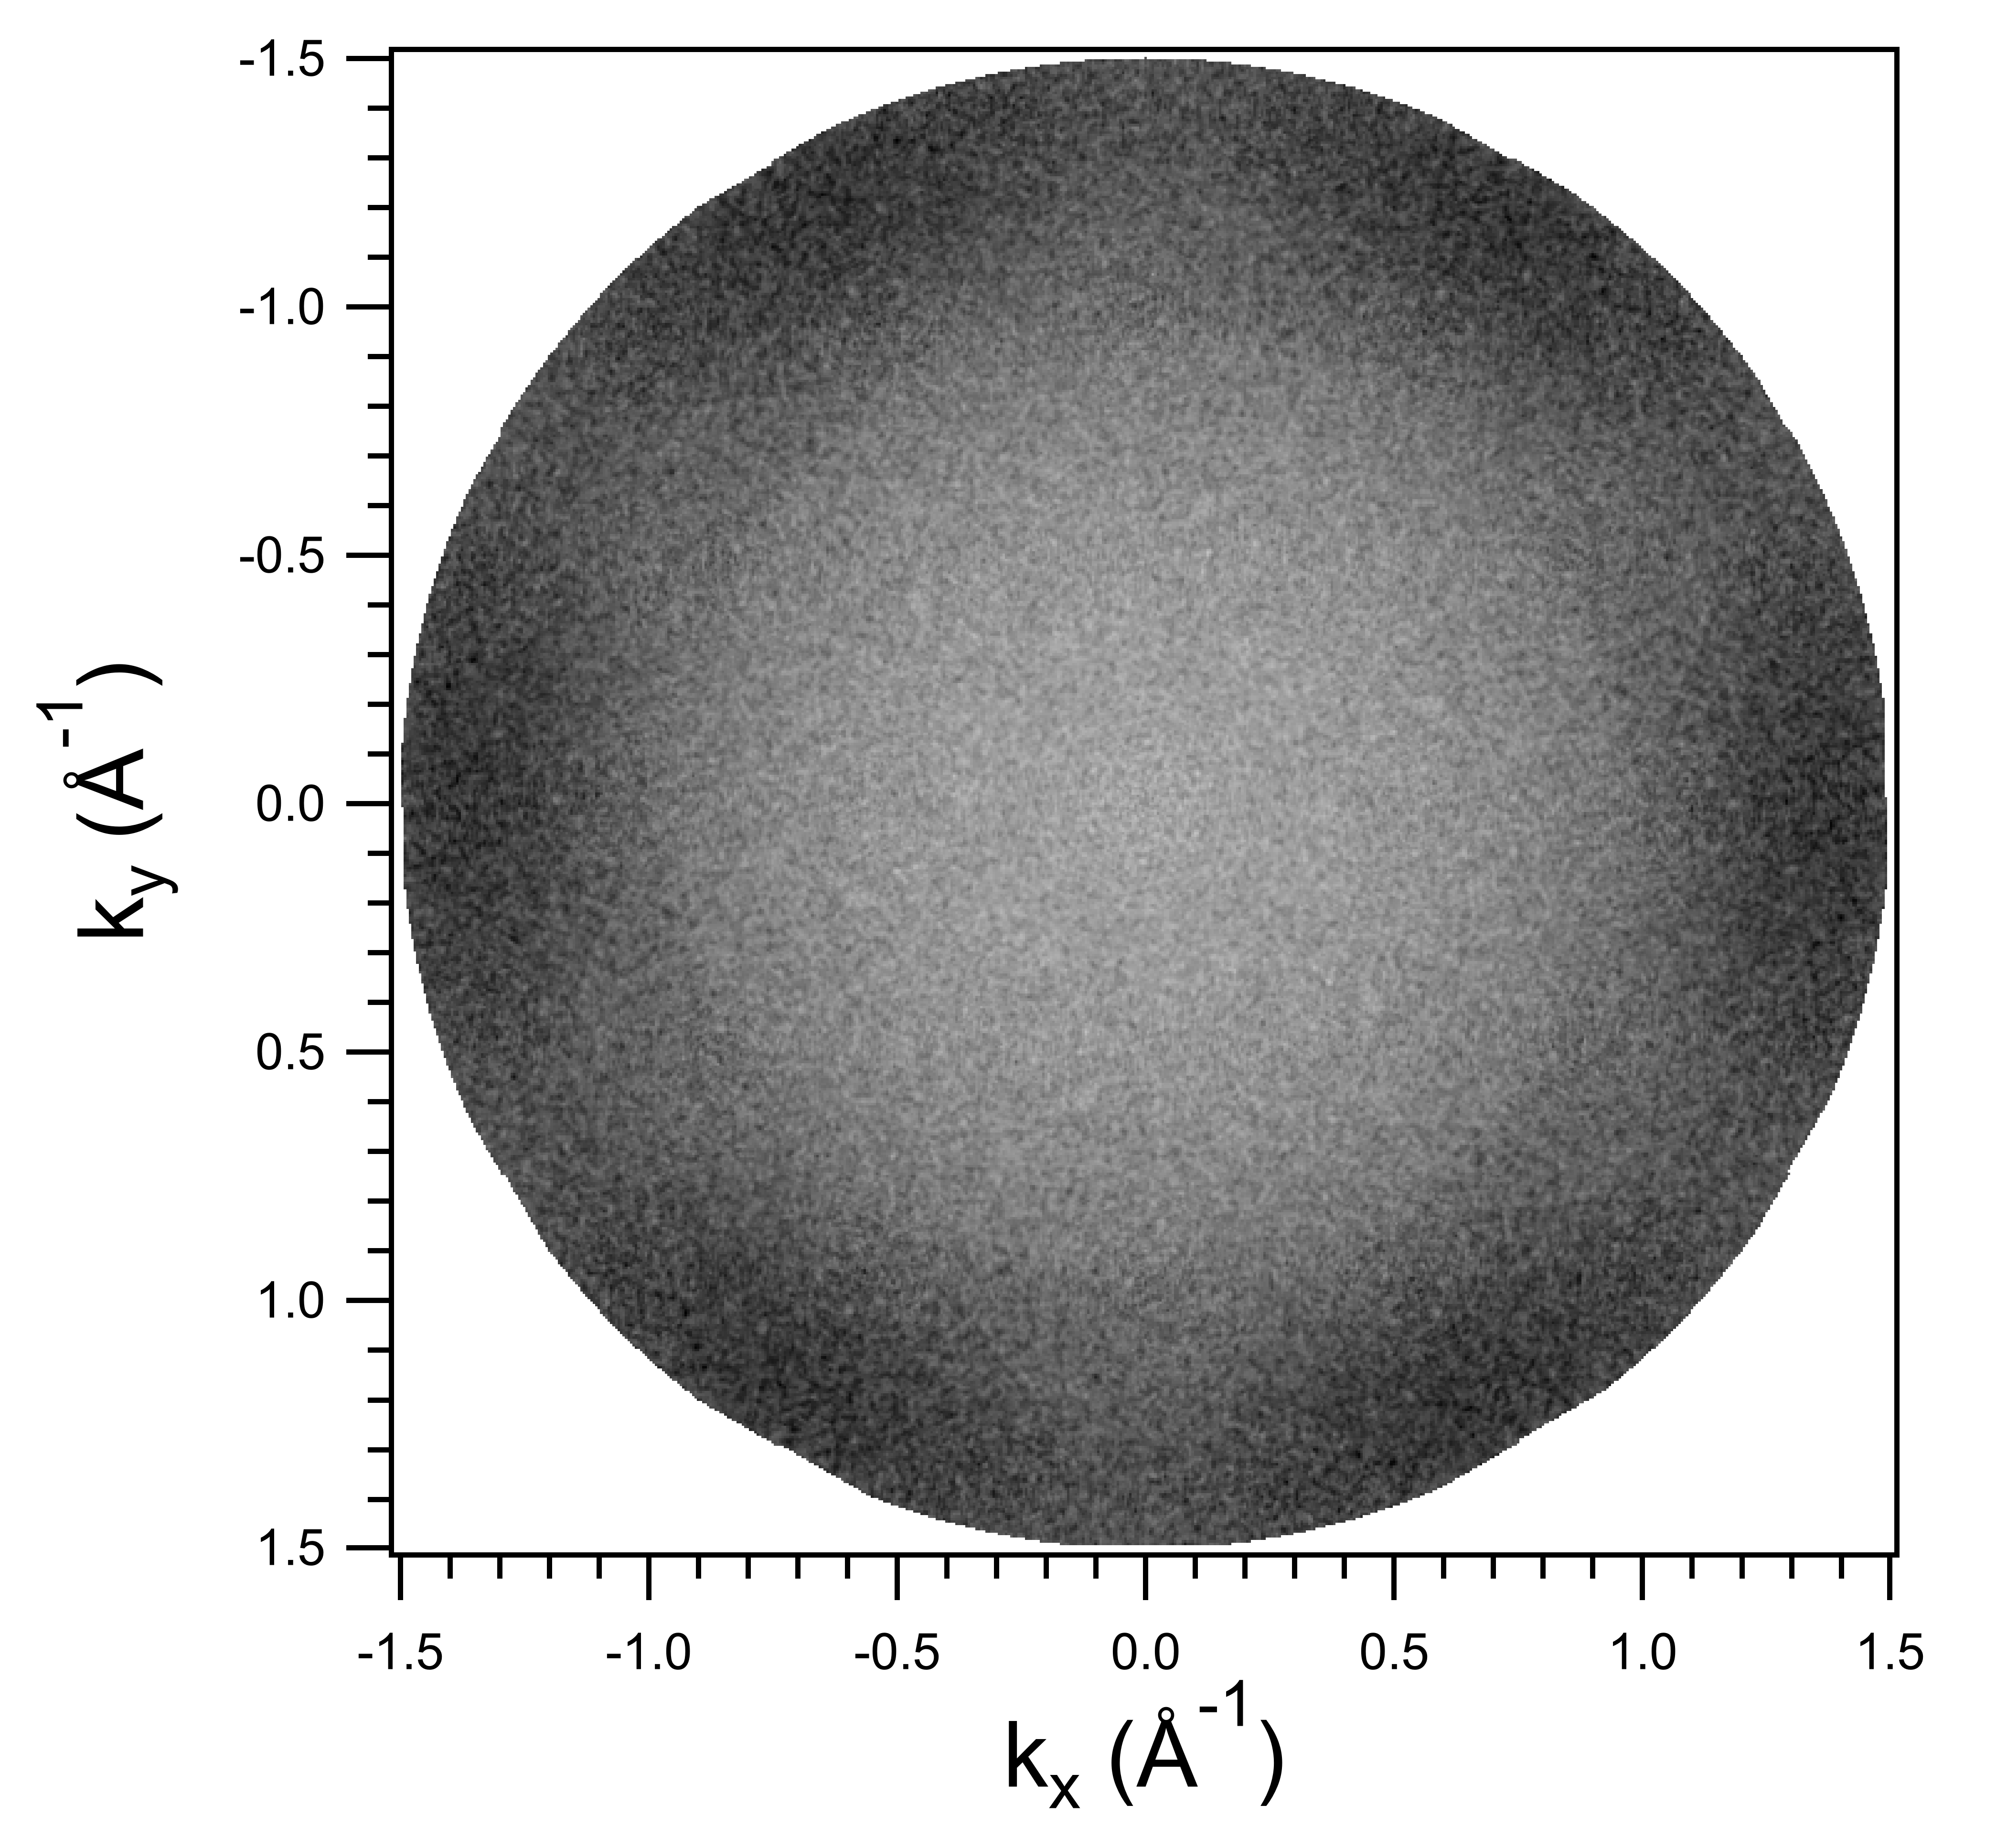
\includegraphics[height=4cm]{Au+5A/MOT_Au_5A_exp_1.png}
                    \subcaption{Gemmesen, symmetrisiertes Bild bei einer Bindungsenergie von \SI{0.8}{\electronvolt}.}
                    \label{fig:MOT_Au+5A_exp_1}
                \end{subfigure}
                \begin{subfigure}[t]{0.48\textwidth}
                    \centering
                    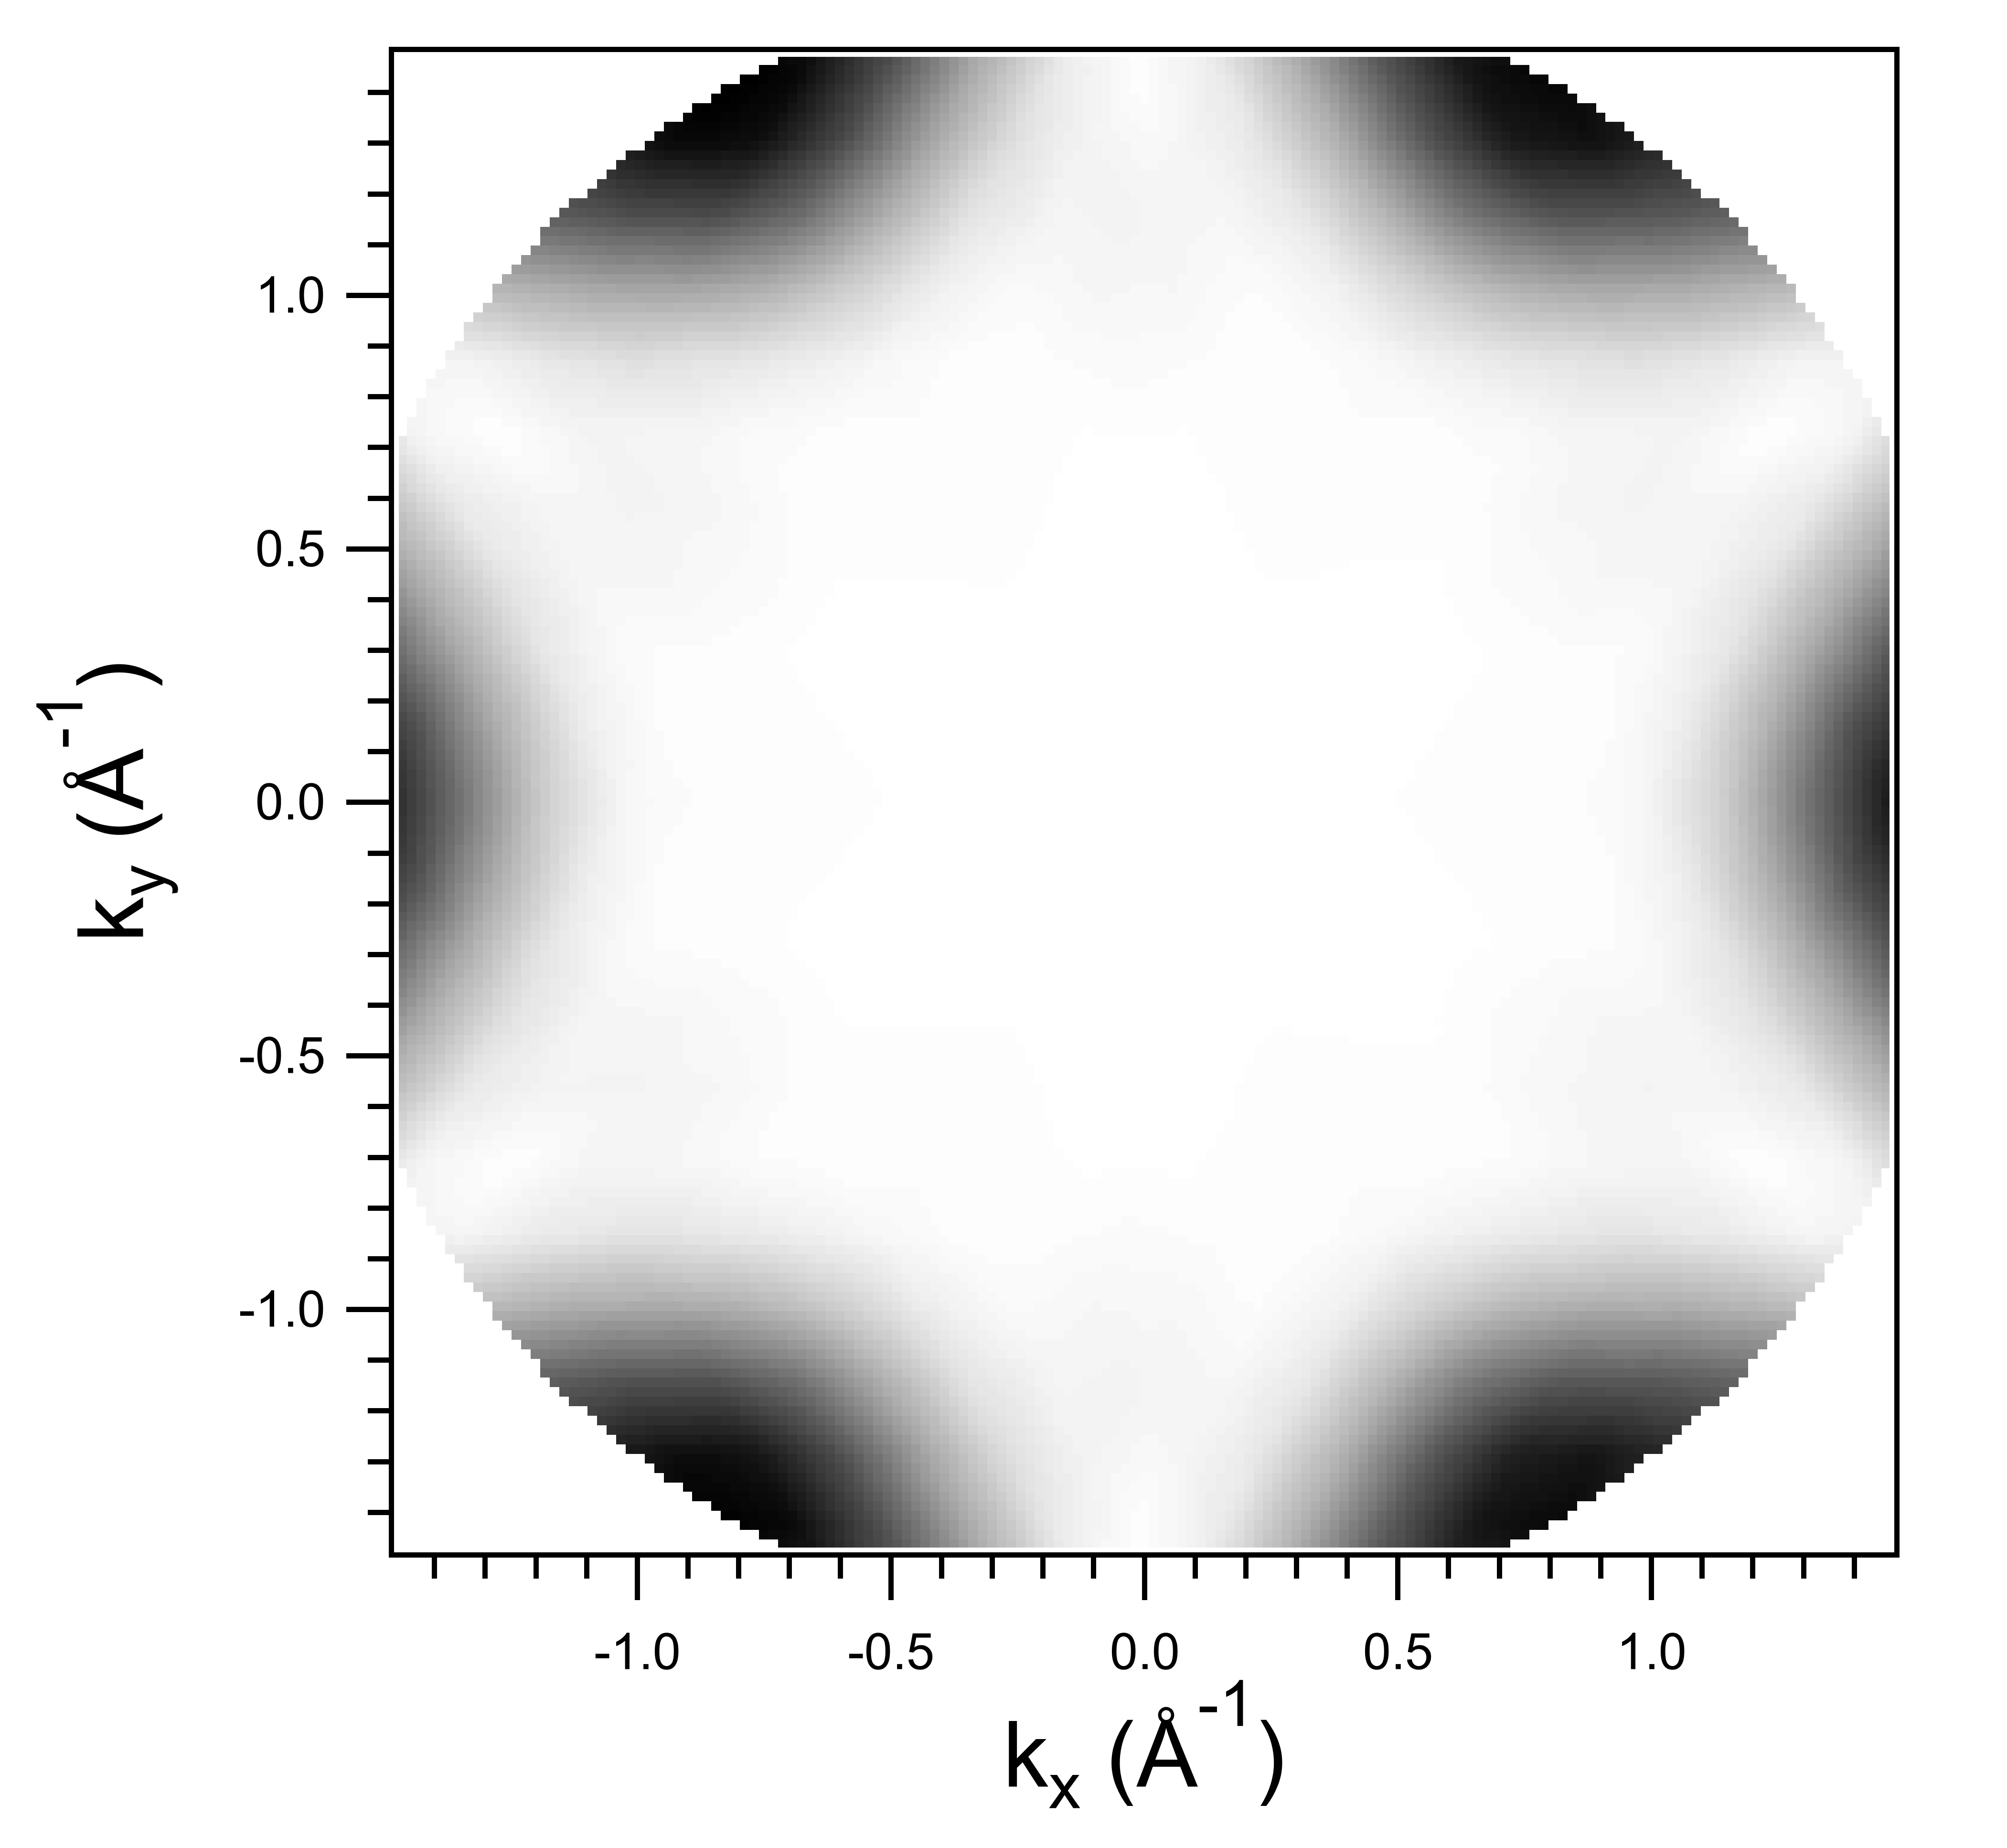
\includegraphics[height=4cm]{Au+5A/HOMO_all_CT}
                    \subcaption{Das theoretisch erwartete HOMO.}
                    \label{fig:MOT_Au+5A_theo_1}
                \end{subfigure}
                \centering
                \begin{subfigure}[t]{0.48\textwidth}
                    \centering
                    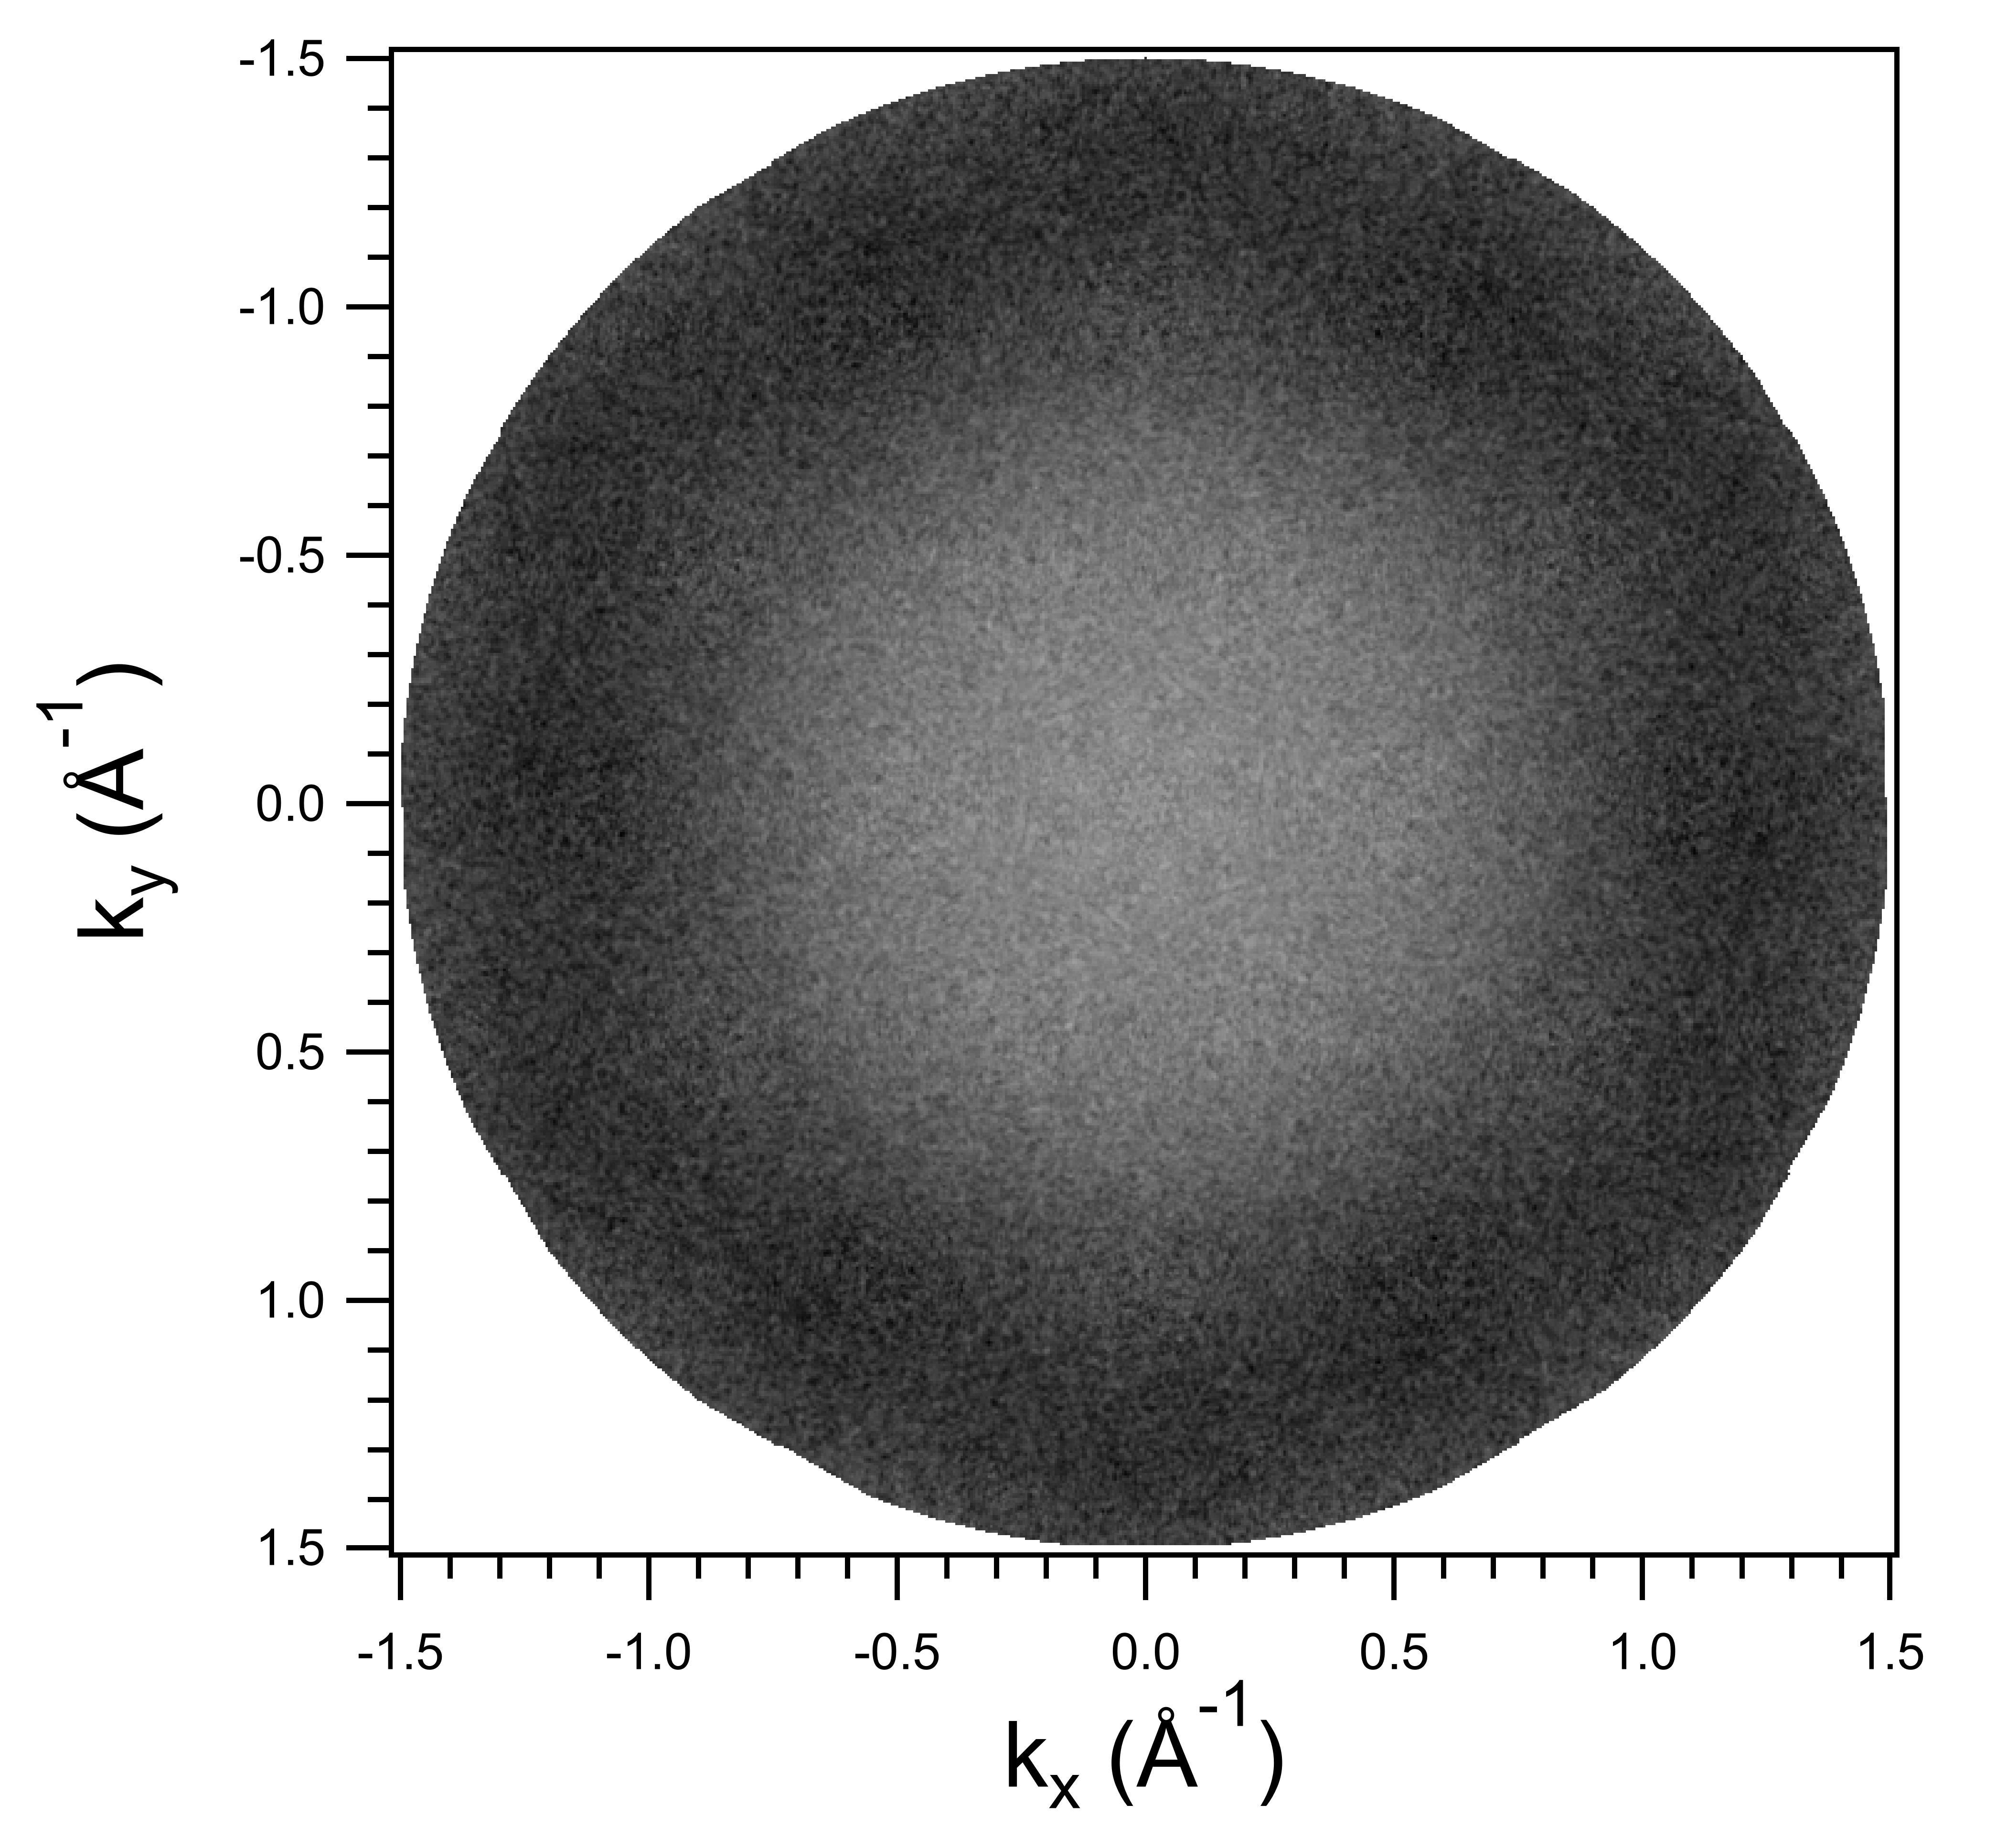
\includegraphics[height=4cm]{Au+5A/MOT_Au_5A_exp_2.png}
                    \subcaption{Gemmesen, symmetrisiertes Bild bei einer Bindungsenergie von \SI{1.85}{\electronvolt}.}
                    \label{fig:MOT_Au+5A_exp_2}
                \end{subfigure}
                \begin{subfigure}[t]{0.48\textwidth}
                    \centering
                    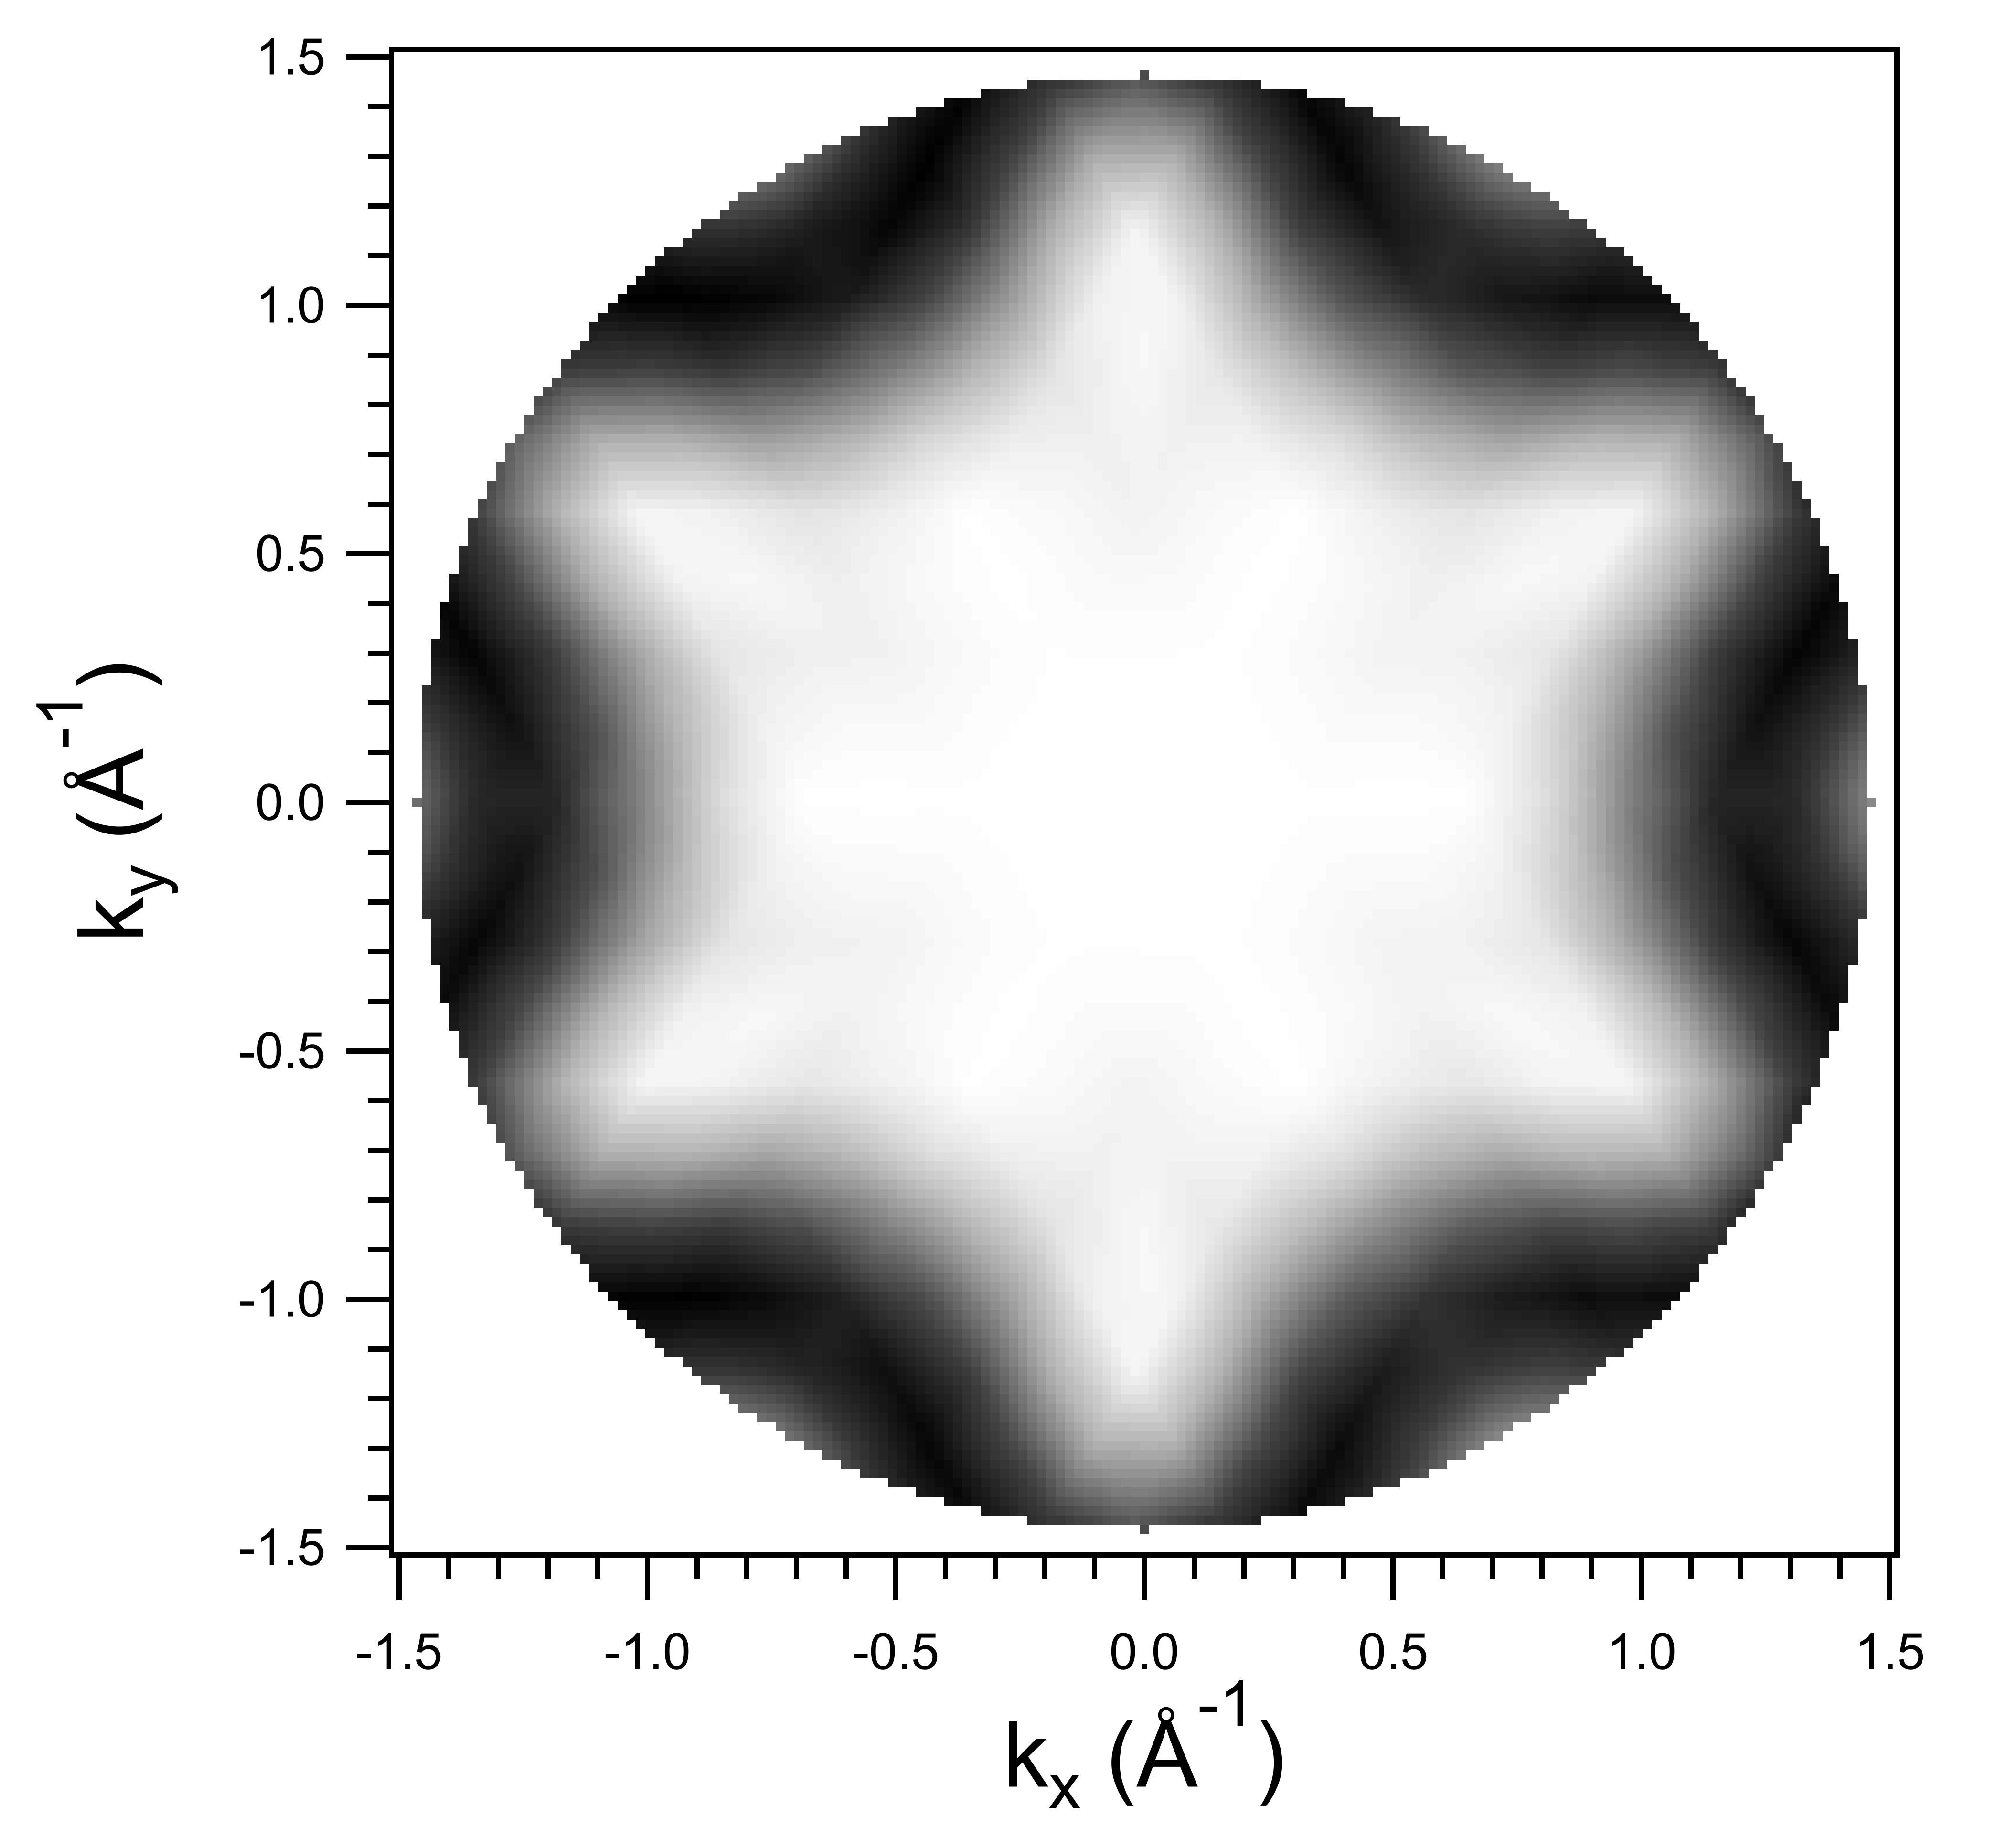
\includegraphics[height=4cm]{Au+5A/HOMO1_all_CT}
                    \subcaption{Theorie Oribtale mit Symmetrisierung des HOMO-1.}
                    \label{fig:MOT_Au+5A_theo_2}
                \end{subfigure}
                \begin{subfigure}[t]{0.48\textwidth}
                    \centering
                    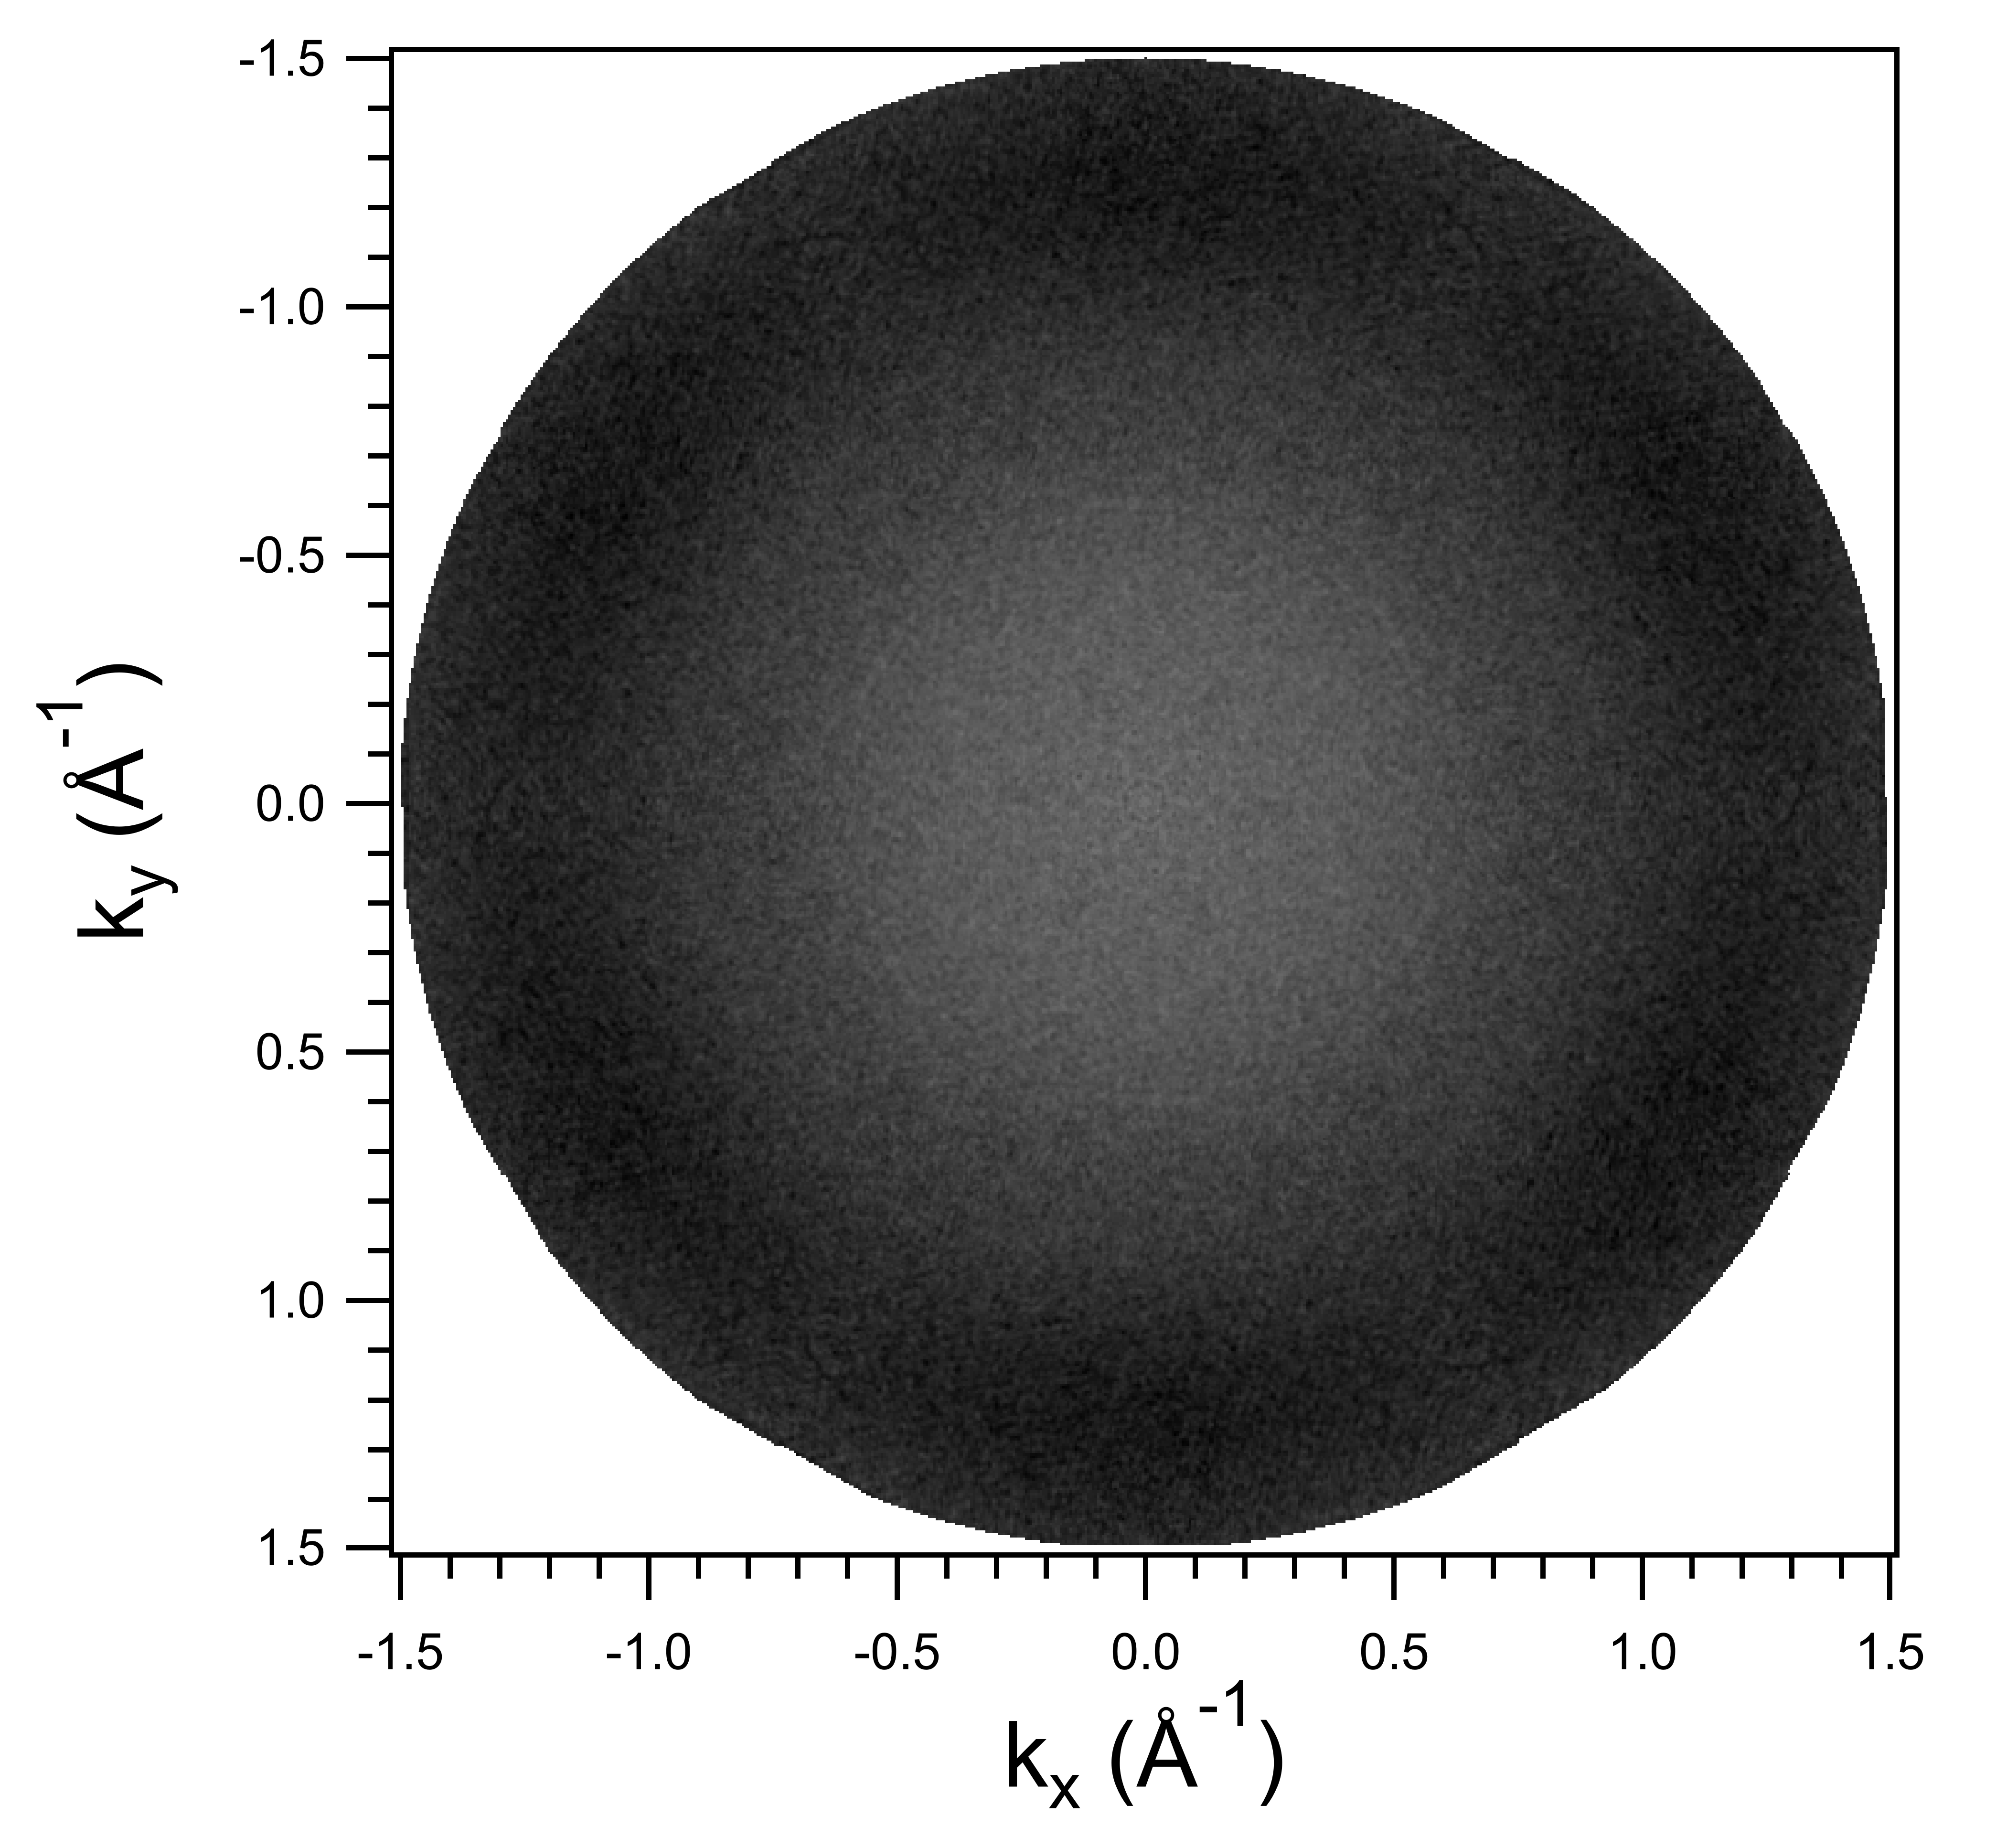
\includegraphics[height=4cm]{Au+5A/MOT_Au_5A_exp_3.png}
                    \subcaption{Gemmesen, symmetrisiertes Bild bei einer Bindungsenergie von \SI{2.65}{\electronvolt}.}
                    \label{fig:MOT_Au+5A_exp_3}
                \end{subfigure}
                \begin{subfigure}[t]{0.48\textwidth}
                    \centering
                    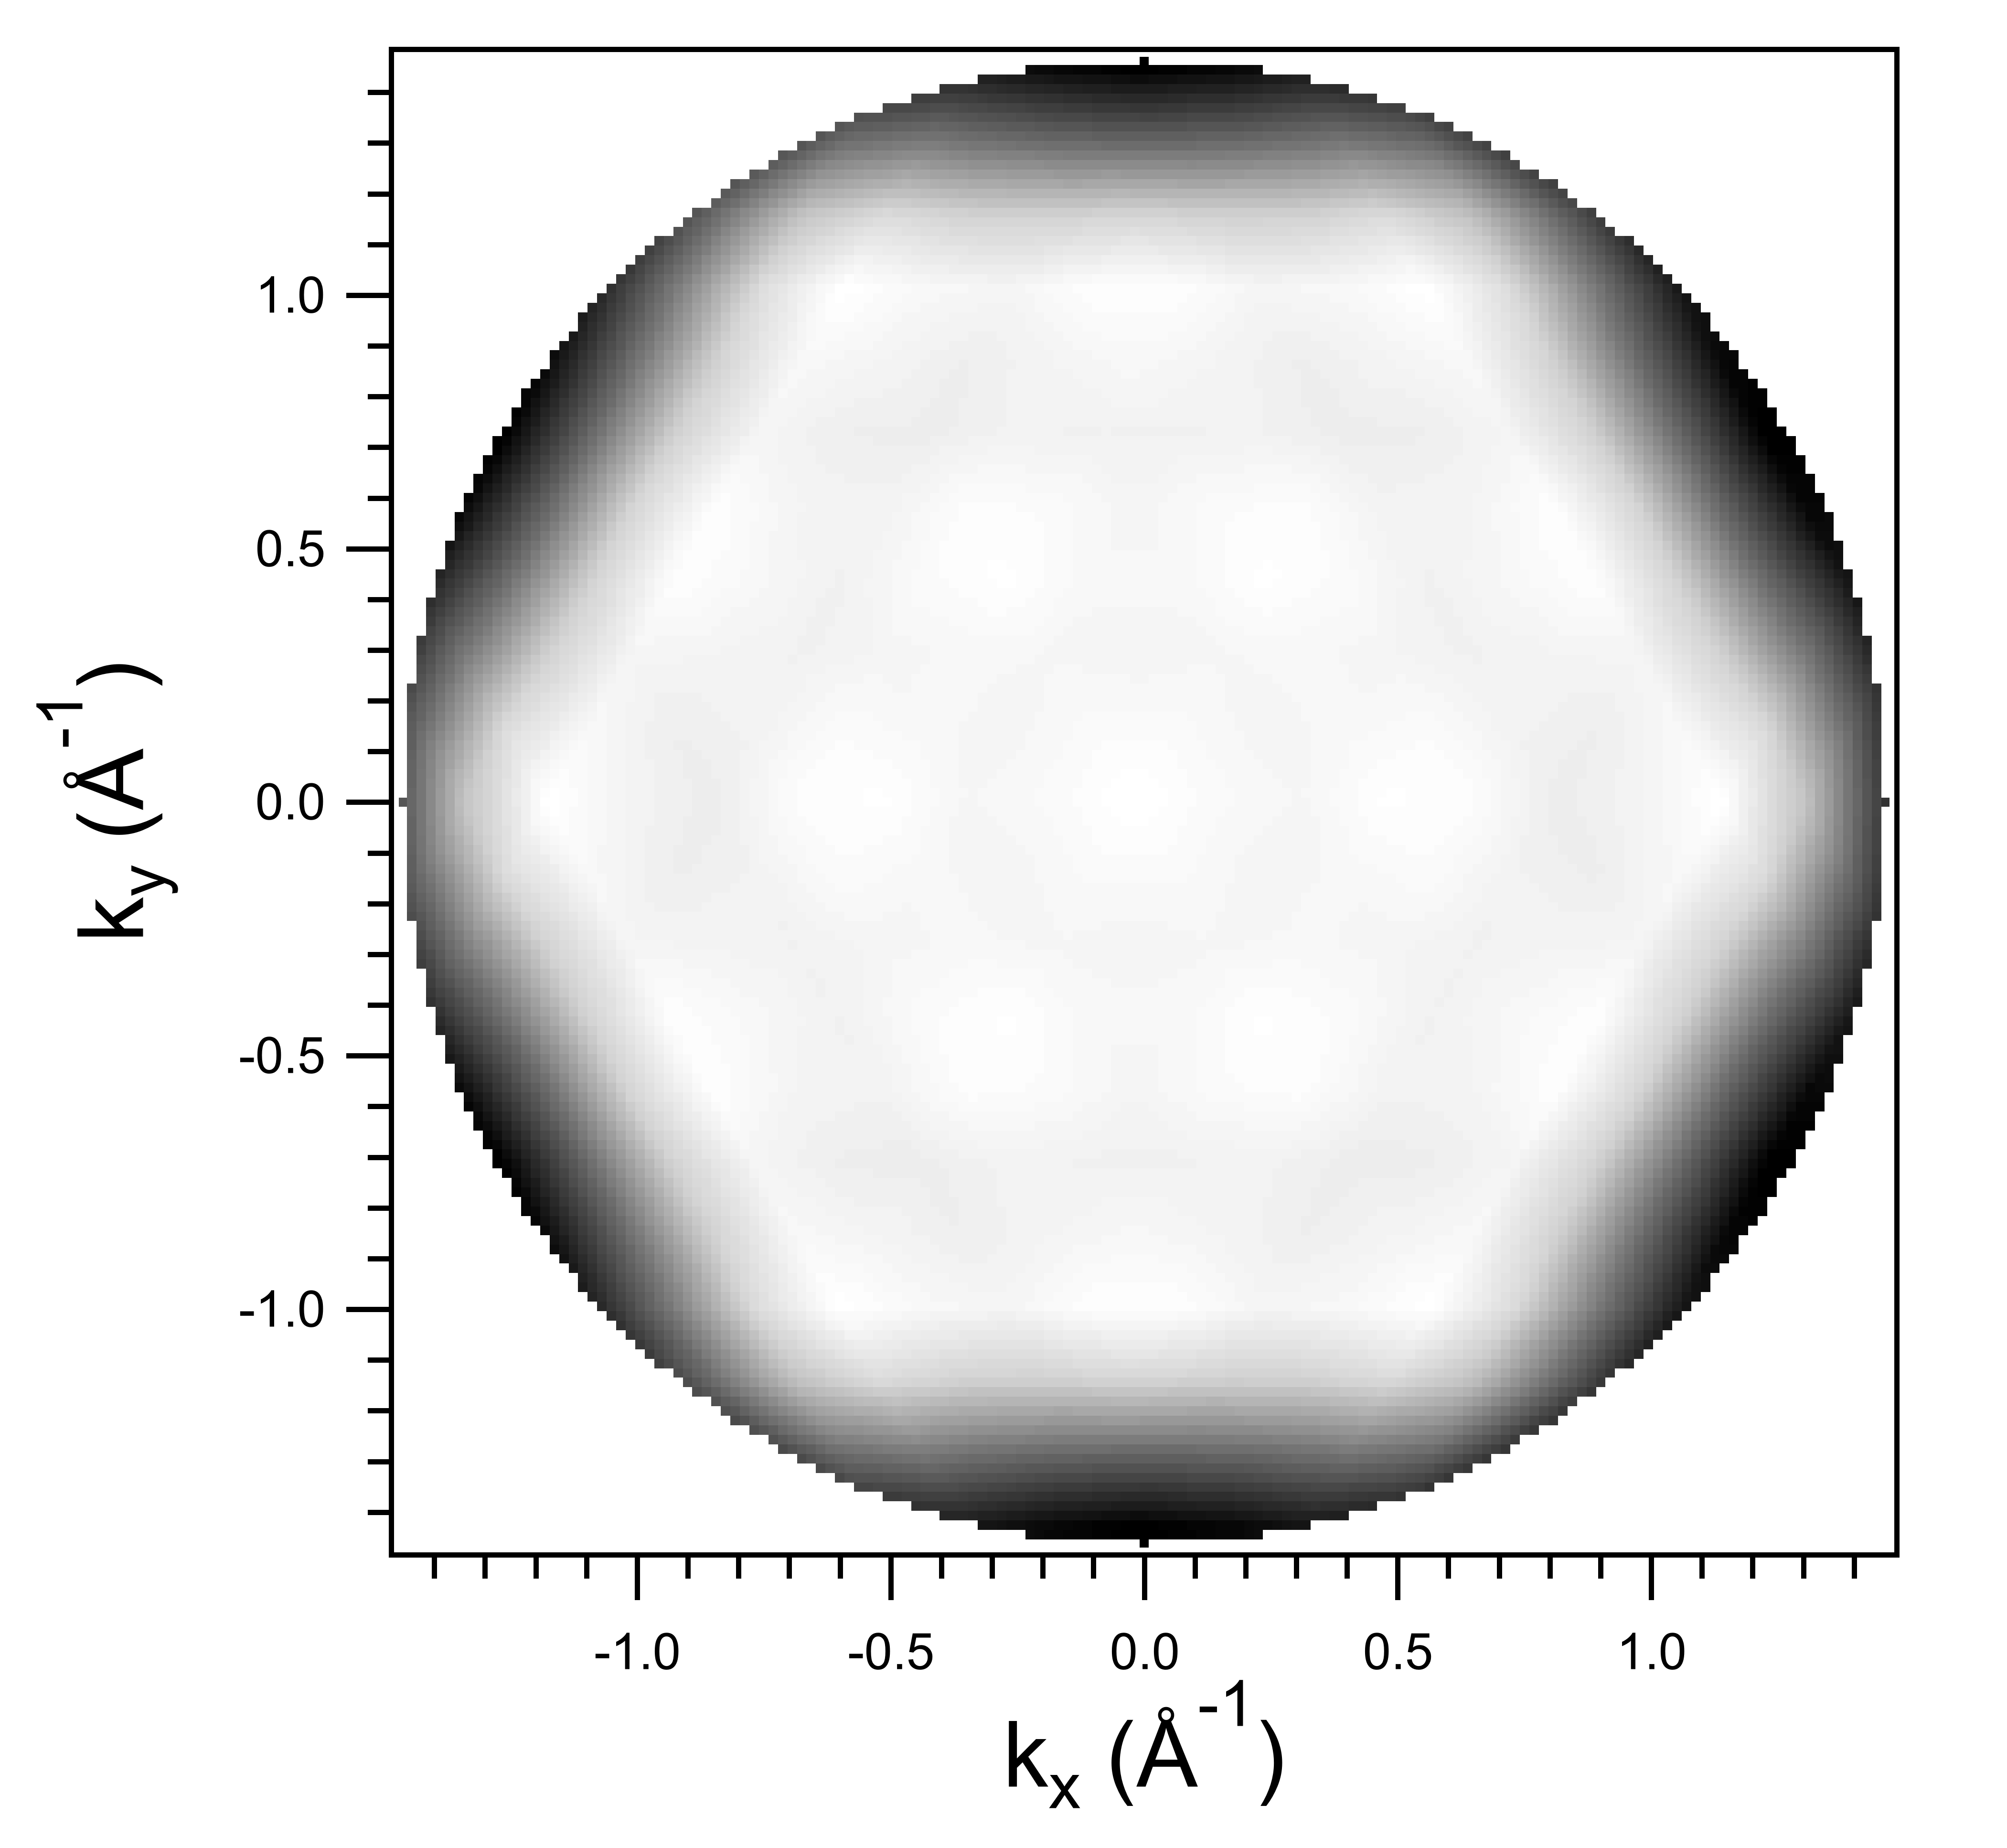
\includegraphics[height=4cm]{Au+5A/HOMO2_all_CT}
                    \subcaption{Berechnetes Theoriebild zum HOMO-2.}
                    \label{fig:MOT_Au+5A_theo_3}
                \end{subfigure}
                \caption{Zuordnung eines Bildes zu einem der Molekülorbitale. Theorie Oribtale mit Symmetrisierung zweimal um 120 Grad gedreht und zum Ursprungsbild addiert.}
                \label{fig:MOT_Au+5A}
            \end{figure}
            Winkelaufgelöste Bilder bei den entsprechenden Energien zeigen auch zusätzliche Merkmale im Bezug zum reinen Gold.
            Gemeinsam mit theoretischen Berechnungen aus der Dichtefunktionaltheorie lassen sich diese dann entsprechenden Molekülorbitalen zuordnen.
            Dies ist für einige Energien und Orbitale in \autoref{fig:MOT_Au+5A} geschehen.
            Dabei wurden die gemessenen wie auch berechneten Bilder entsprechend der Geometrie aus dem Beugungsbild \autoref{fig:LEED_Au+5A} jeweils um \SI{120}{\degree} gedreht und aufsummiert.
    
            Eine Zuordnung einer der markanten Elemente zu einem zuvor unbestzten Orbital, dem LUMO ist nicht zu erkennen.
            Es scheint also so als würden keine Elektronen zwischen Substrat und Molekül ausgetauscht werden. 
            Dies lässt sich auch aus der Literatur erkennen, dass sich bei den Anornung von Pentacene auf Gold um den Prozess der Physisorption handelt~\cite{5A_4}.
            Abwesenheit des LUMOs in den Spektren und Bildern muss aber nicht zwangsläufig auf die Physisorption hindeuten.
            So ist Pentacene auf Kupfer (111) chemisch adsorbiert und zeigt dennoch keine Anzeichen der Besetzung des LUMO~\cite{koch_adsorption-induced_2008}.

            \section{Sonstiges}
            \begin{itemize}
                \item Die mittlere freie Weglänge $\lambda$ ist die in der \SI{63}{\percent} der Elektronen Energieverlust erfahren \cite{vickerman_surface_2009}
                \item VB Spektrum UPS zeigt 'alles' und XPS VB mehr die Metalle!
            \end{itemize}

            \subsection{XMCD/XMLD}
            Neben der Abhänigkeit von der Photonenenergien ist die Absorption auch von der Polarisation des Lichts selbst abhängig.
            So lässt sich aus den Unterschieden der Absorptionsintensitäten für s- und p-polarisiertem Licht die Neigung von Molekülen auf der Oberfläche kalkulieren\cite{floreano_periodic_2008}.
            Ebenso wird durch die Ausrichtung der magetischen Momente die Orbitalstruktur ebenfalls in diese Richtung gestreckt.
            Nun kommt der Polarisationfaktor für den Photoemissionsstrom zu tragen.
            Sind Polarisation der Photonen und Orbitalgeometrie parallel gerichtet kommt es zur verstärkten Absorption, im Gegensatzt dazu, wenn diese senkrecht aufeinander stehen.
            Aus der Differenz der beiden Anteile ergibt sich dann das Signal der Röntgen linear magnetischer Dichroismus (XMLD, \textit{X-ray magnetic linear dichroism}).
            Dieser Effekt tritt für antiferromagnetisch wie auch für ferromagnetisch Materialien auf.
            Für zirkularpolarisiertes Licht ergibt sich aus dem Intensitätsunterschied der links- und rechtszirkularpolarisertem Licht die Magnetisierung für ferromagnetisch Materialien.
            Durch die unterschiedelichen Polarisationen wird die eine oder andere Spinsorte vermehrt angeregt.
            An der Fermikante sind nur Zustände einer gewissen Spinsorte unbesetz.
            Da ein Spinflip verboten ist, dienen diese Zustände als Detektor für den Spin der angeregten Elektronen~\cite{stohr_magnetism_2006}.

            \subsection{Wüstit}
            \begin{figure}
                \centering
                \begin{subfigure}[t]{0.48\textwidth}
                    \centering
                    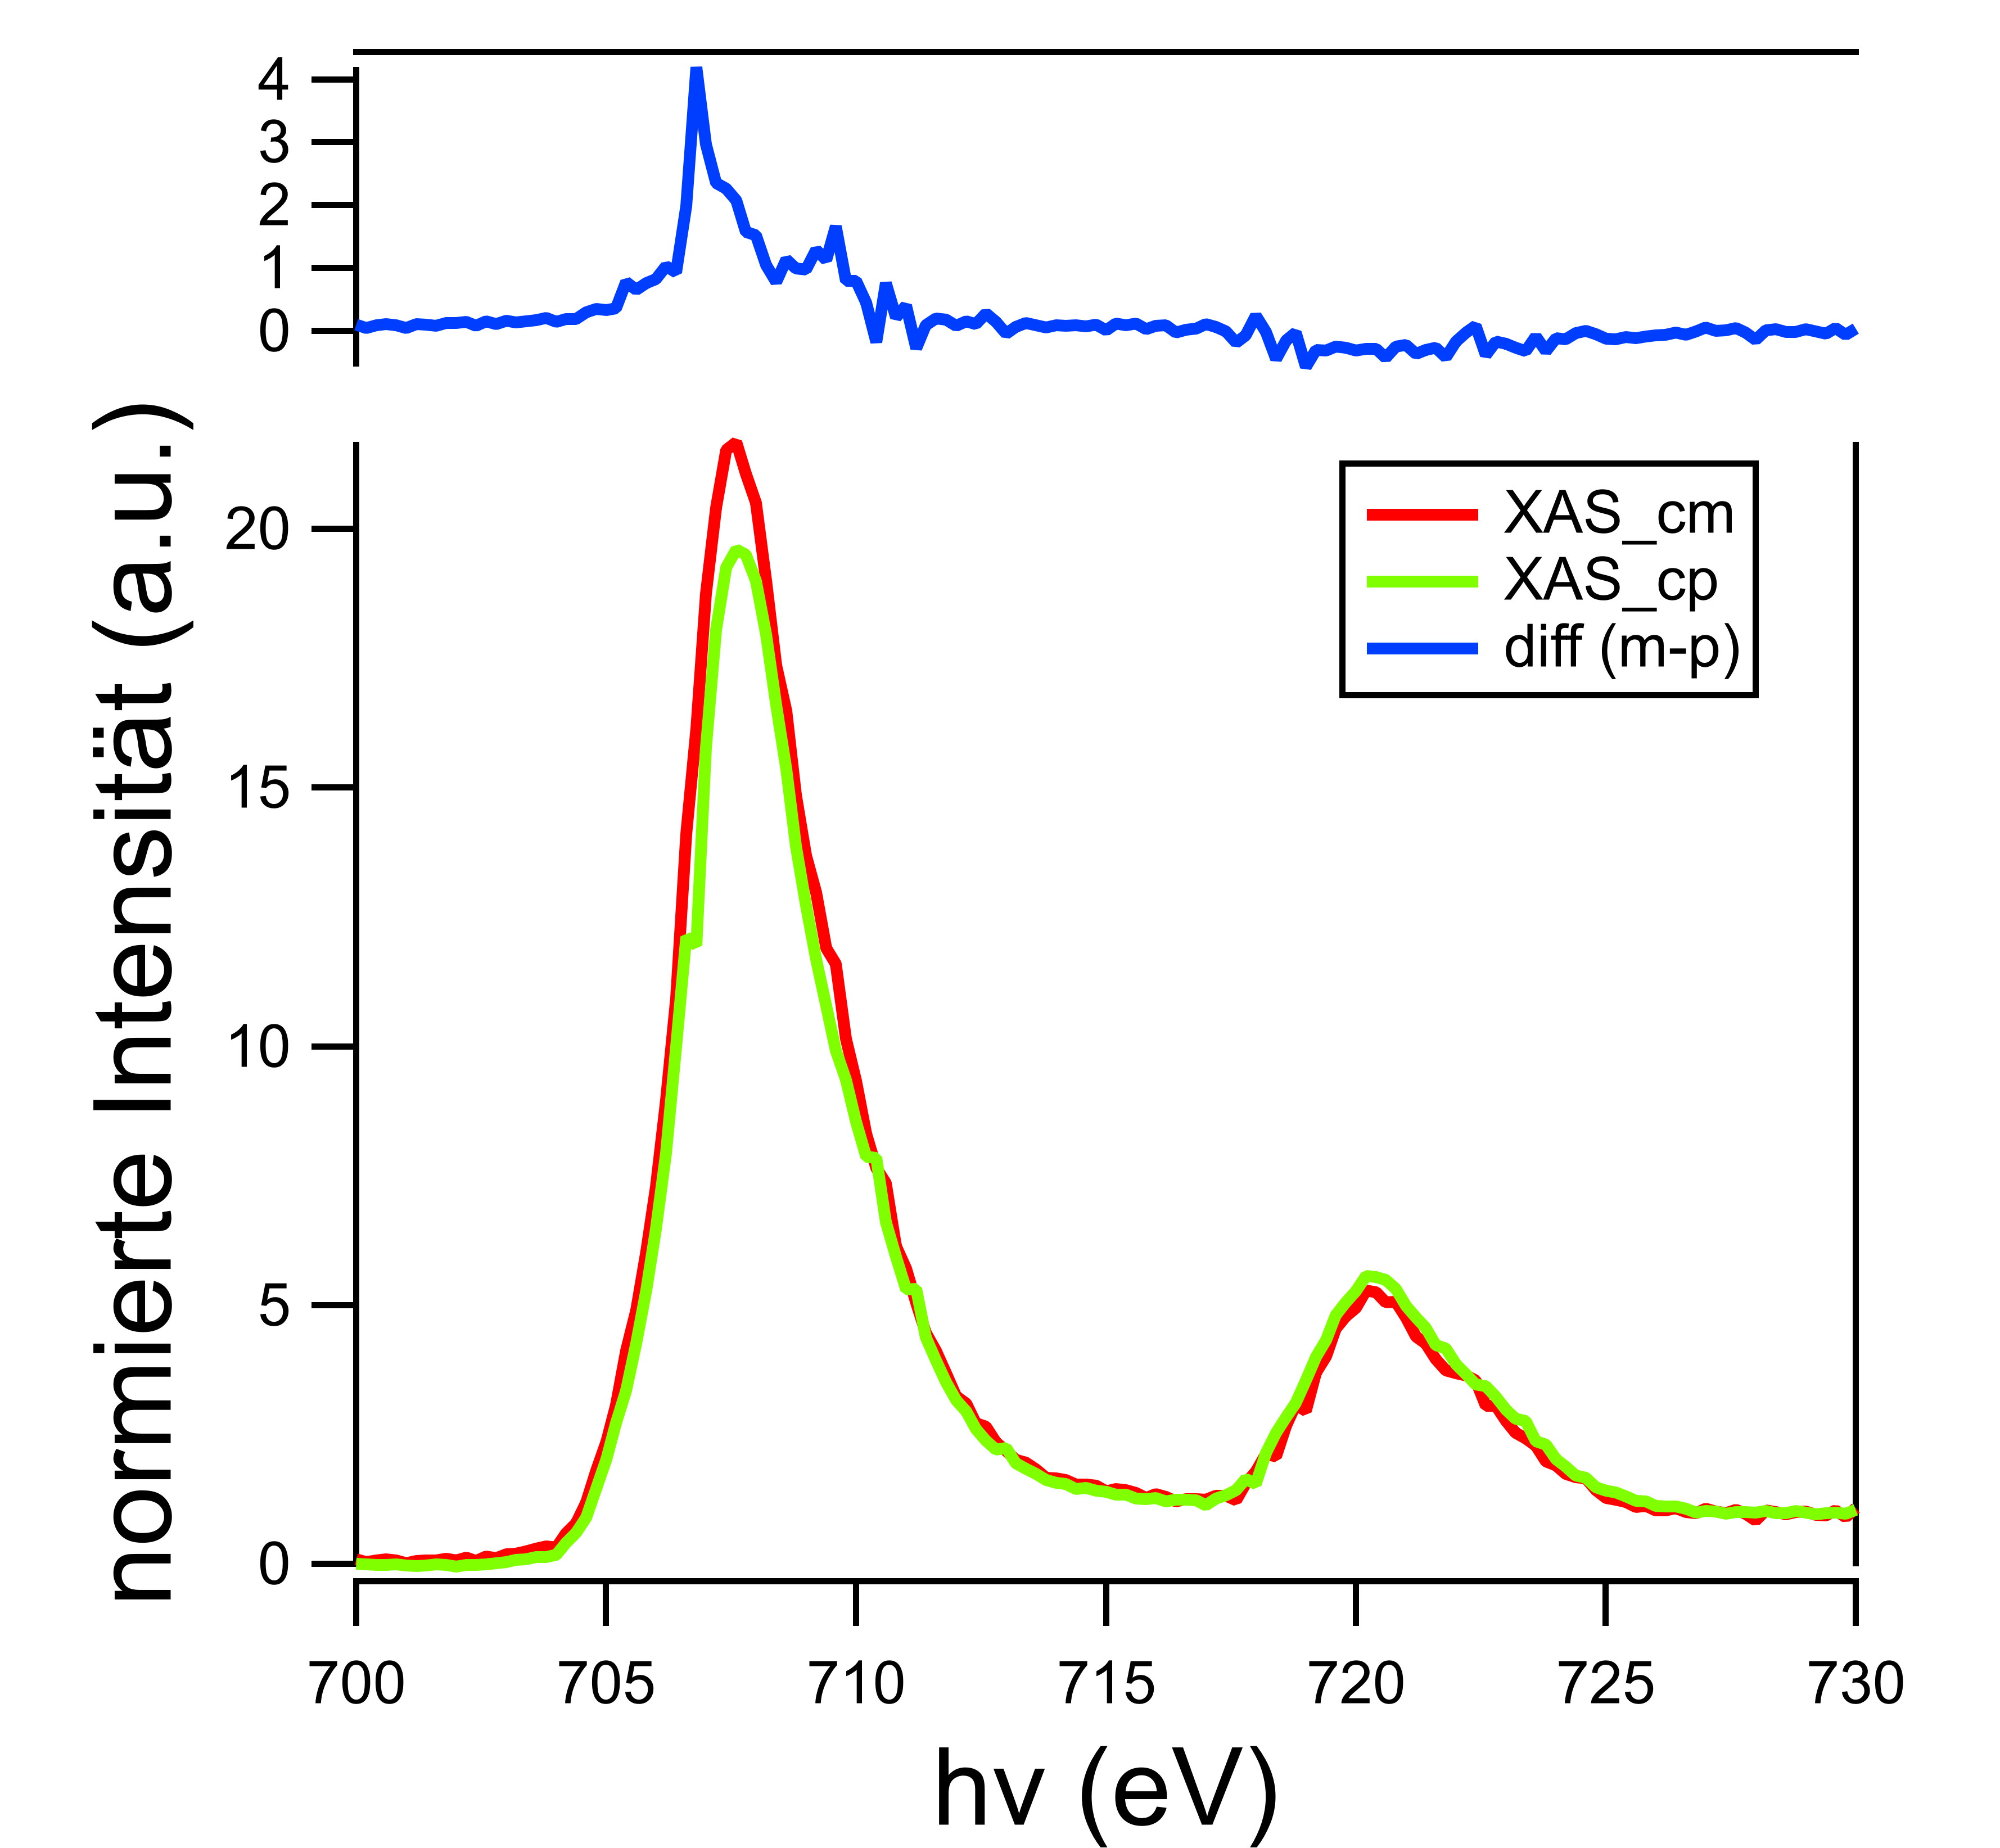
\includegraphics[height=5cm]{FeO/XMCD_FeO.png}
                    \caption{Spektren für links- und rechtzirkular polarisiertes Licht und ihre Differenz dem XMCD Signal.}
                    \label{fig:XMCD}
                \end{subfigure}
                \begin{subfigure}[t]{0.48\textwidth}
                    \centering
                    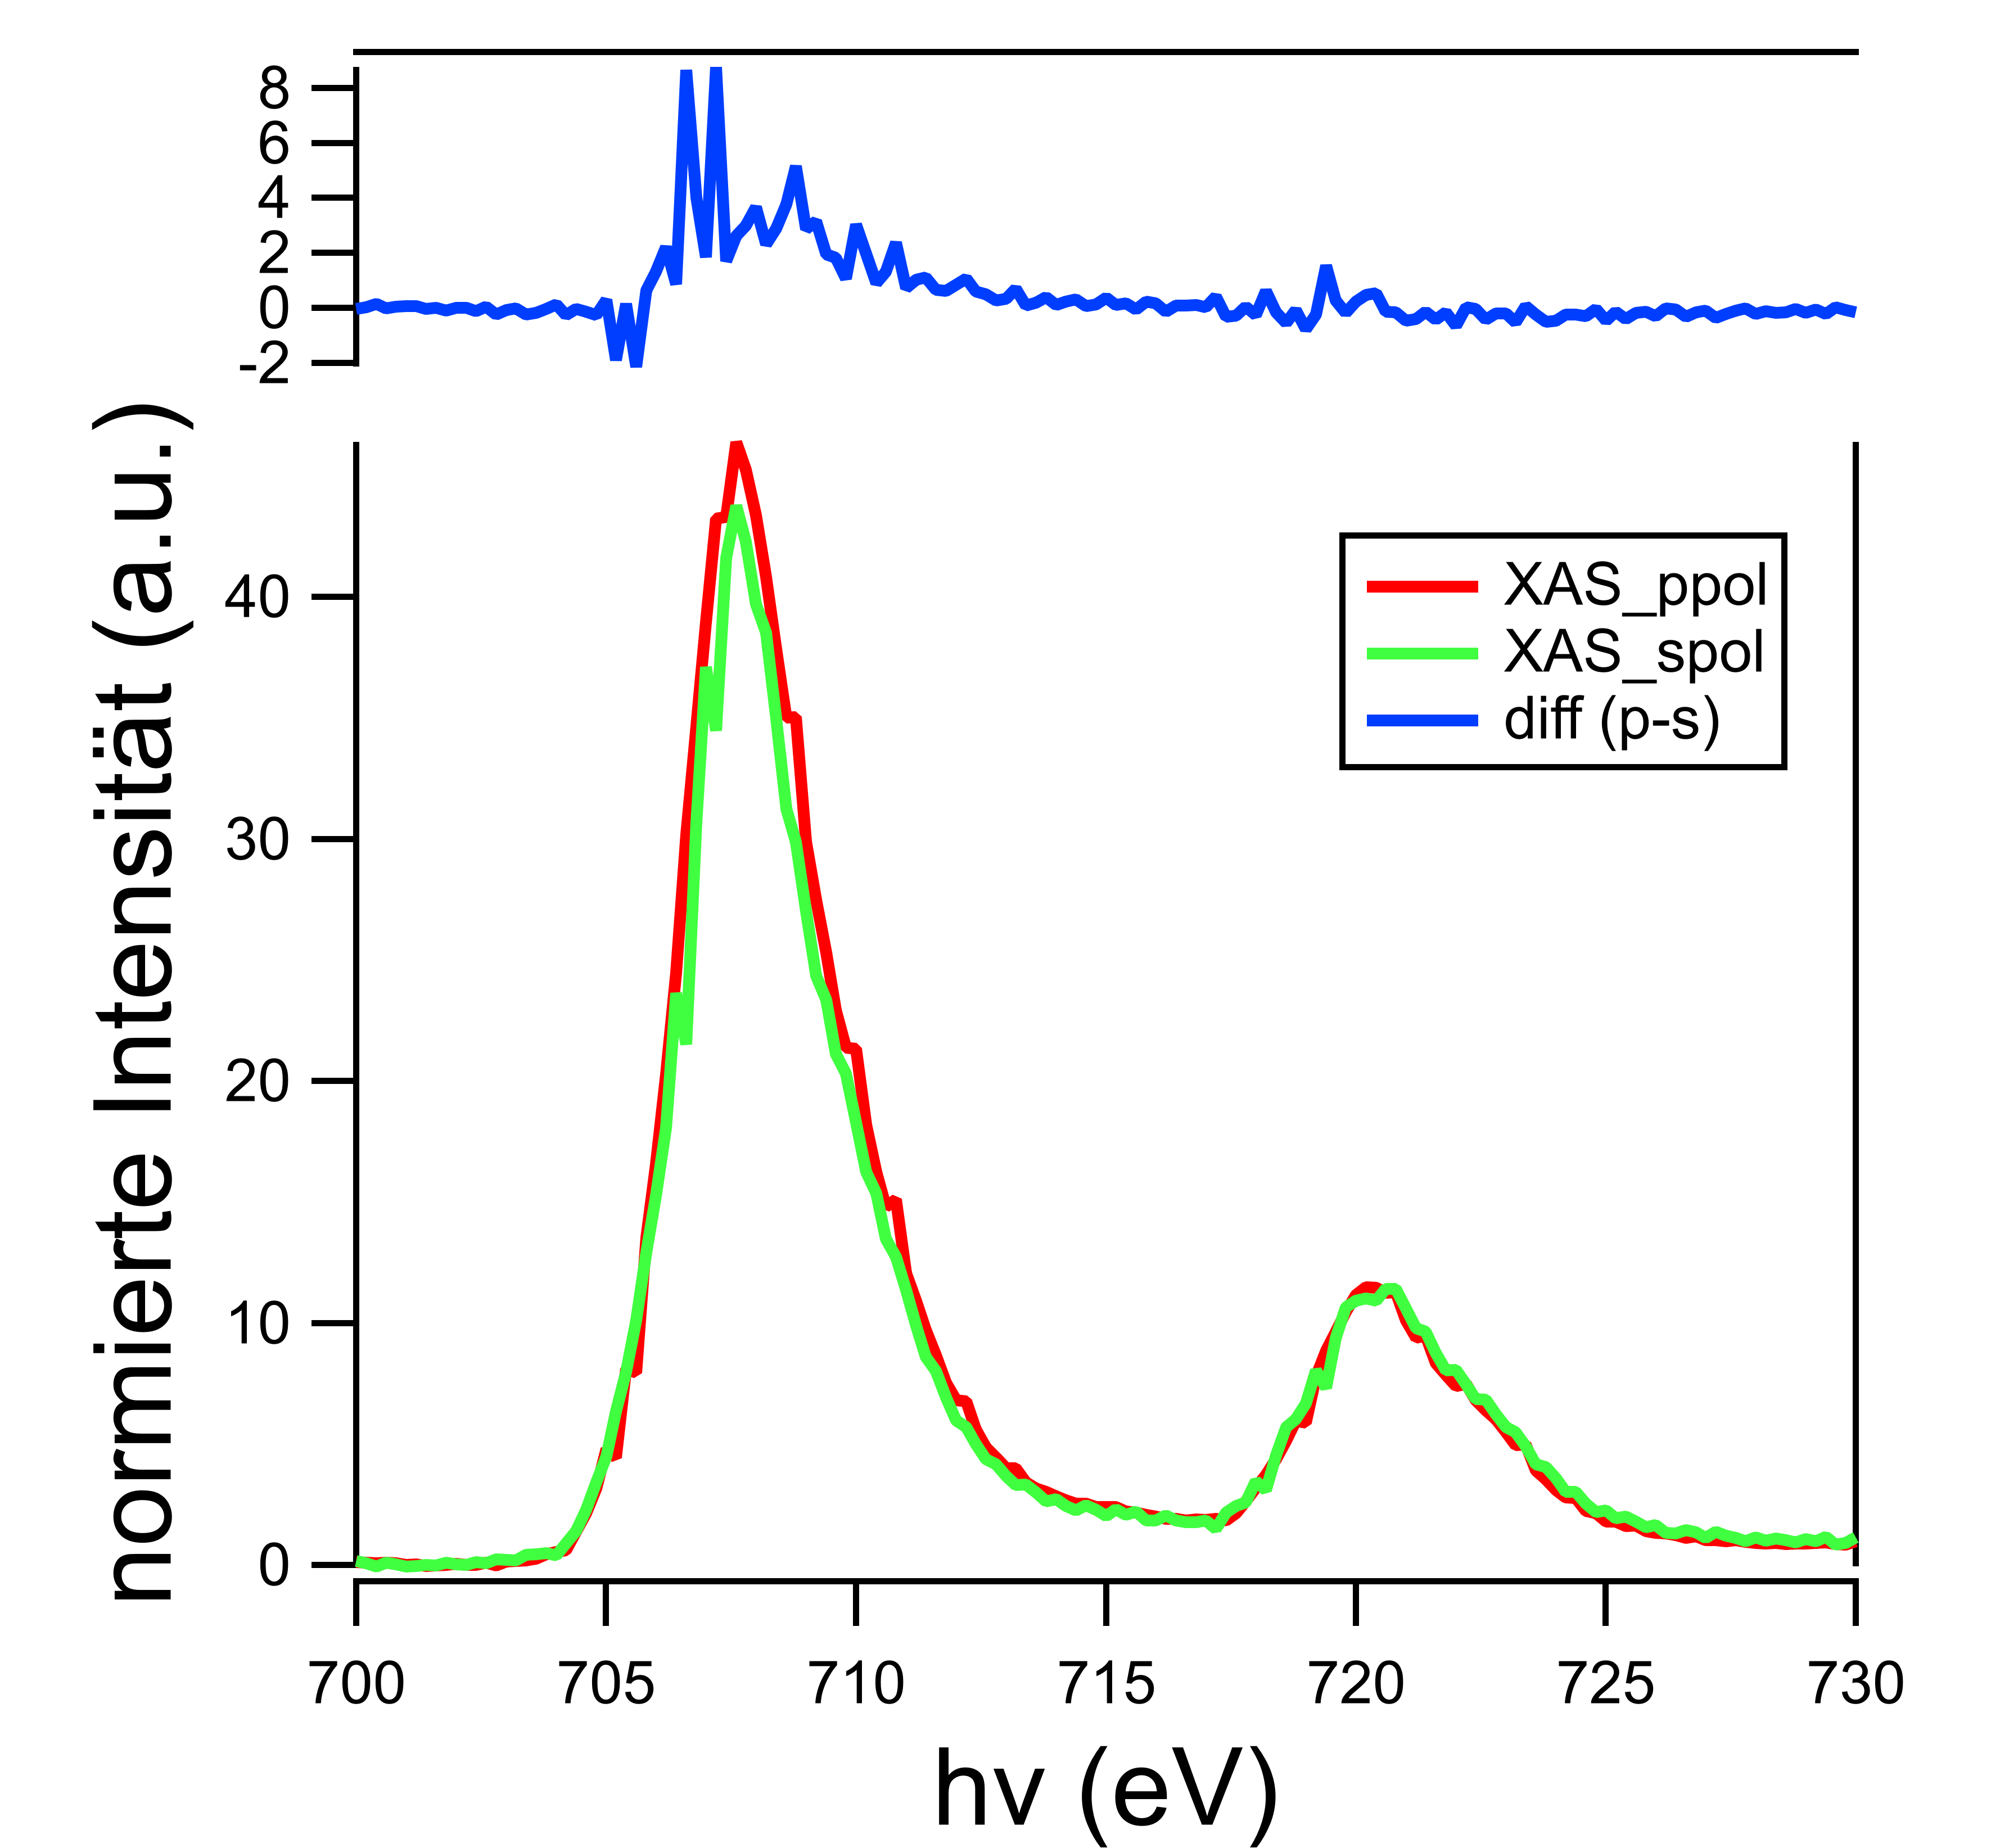
\includegraphics[height=5cm]{FeO/XMLD_FeO.png}
                    \caption{Spektren für s- und p- polarisiertes Licht, sowie dessen Differenz dem XMLD Signal.}
                    \label{fig:XMLD}
                \end{subfigure}
                \caption{Die verschiedenen XAS Messungen mit unterschiedlichen Polarisationen. Aus der Differenz ergeben sich dann die XMCD und XMLD Signale.}
                \label{fig:XAS_FeO}
            \end{figure}
            Mit Hilfe des magnetischen Röntgen-Zirkular-Dikorismus und magnetischen Röntgen-Linear-Dikorismus lassen sich die magnetischen Eigeschaften des Substrates untersuchen.
            Beide Spektren der Röntgenabsorptionsmessungen sind in \autoref{fig:XAS_FeO} zu sehen.
            \begin{itemize}
                \item Das XMCD Signal sollte für L3 und L2 umegkehrt sein, wenn es Ferromagnetisch ist, Signal lässt sich aber nur bei L3 erkennen.
                \item Auch XMLD für Antiferromagnetismus auf Grund der nicht spärischen Oribtale durch die Spin-Bahn-Kopplung (Spins ausgerichtet) \cite{stohr_magnetism_2006} - kann auch eben sein, dass die Spins nicht ausgerichtet waren. T war unter Neel Temperatur.
                \item Eventuell kein XMLD Signal, falls Probe nicht geordnet oder viele Domänen aufweist. Die Easy-Axis des Fe lag auch genau 45° zu p und s.
                \item Kleine XMLD Effekte können auch durch die Liganden zu stande kommen, da diese ja auch das Orbital verformen können (besser T abhänig messen)
                \item Warum kein XMCD und XMLD Signal? Es bilden sich Domänen mit einer Größe von \SIrange{50}{500}{\nano\meter} aus. Diese müssen erst durch ein hinreichend großes Feld ausgerichtet werden. Ansonsten haben die Domänen alle Magnetisierungen in unterschiedliche Richtungen. \cite{cornell_iron_2003}

            \end{itemize}